\documentclass[11pt, letterpaper, twoside]{article}
\usepackage[utf8]{inputenc}
\usepackage[T1]{fontenc}
\usepackage{fancyhdr}
\usepackage[margin=1in, include foot]{geometry}
\usepackage{ragged2e}
\usepackage[]{hyperref}
\usepackage{apacite}
\usepackage{setspace}
\usepackage{caption}
\usepackage{subcaption}
\usepackage{etoolbox}
\usepackage{graphicx}
\usepackage{amsmath, amssymb}
\usepackage{cleveref}
\usepackage{wrapfig}
\usepackage{afterpage}
\usepackage{floatrow}
\usepackage{tikz}
\usepackage{booktabs}
\usepackage{siunitx}
\usepackage{dcolumn}
\usepackage{pdflscape}
\usepackage{adjustbox}
\usepackage{tablefootnote}



\setlength{\parindent}{0pt}
\floatsetup[table]{capposition=top}

\title{\singlespacing\textbf{Capture of the Academic Industrial Organization Literature}}


\author{ 
    Joshua Y. Levy \thanks{Joshua Y. Levy  (joshua.levy@chicagobooth.edu), Stigler Center, Booth School of Business, University of Chicago}}
\date{\today}

\onehalfspacing
\begin{document}
\begin{titlepage}
    \maketitle
    \thispagestyle{empty}
\end{titlepage}


\newpage
\pagenumbering{arabic}


\section{The Production of Academic Articles}
Between 1991 and 2020, the amount of space for articles in the Top 5 journals, the \textit{American Economic Review} (AER), \textit{Econometrica} (ECA), the \textit{Journal of Political Economy} (JPE), the \textit{Quarterly Journal of Economics} (QJE), and the \textit{Review of Economic Studies} (RES) (and the \textit{RAND Journal of Economics} (RJE)) has grown slowly and steadily. Notably, however the AER makes up some 40\% of articles published in the Top 5, with almost double the number of articles that any other journal published in any given year.\\
\begin{figure}[!ht]
    \begin{subfigure}[h]{0.49\textwidth}
        \centering
        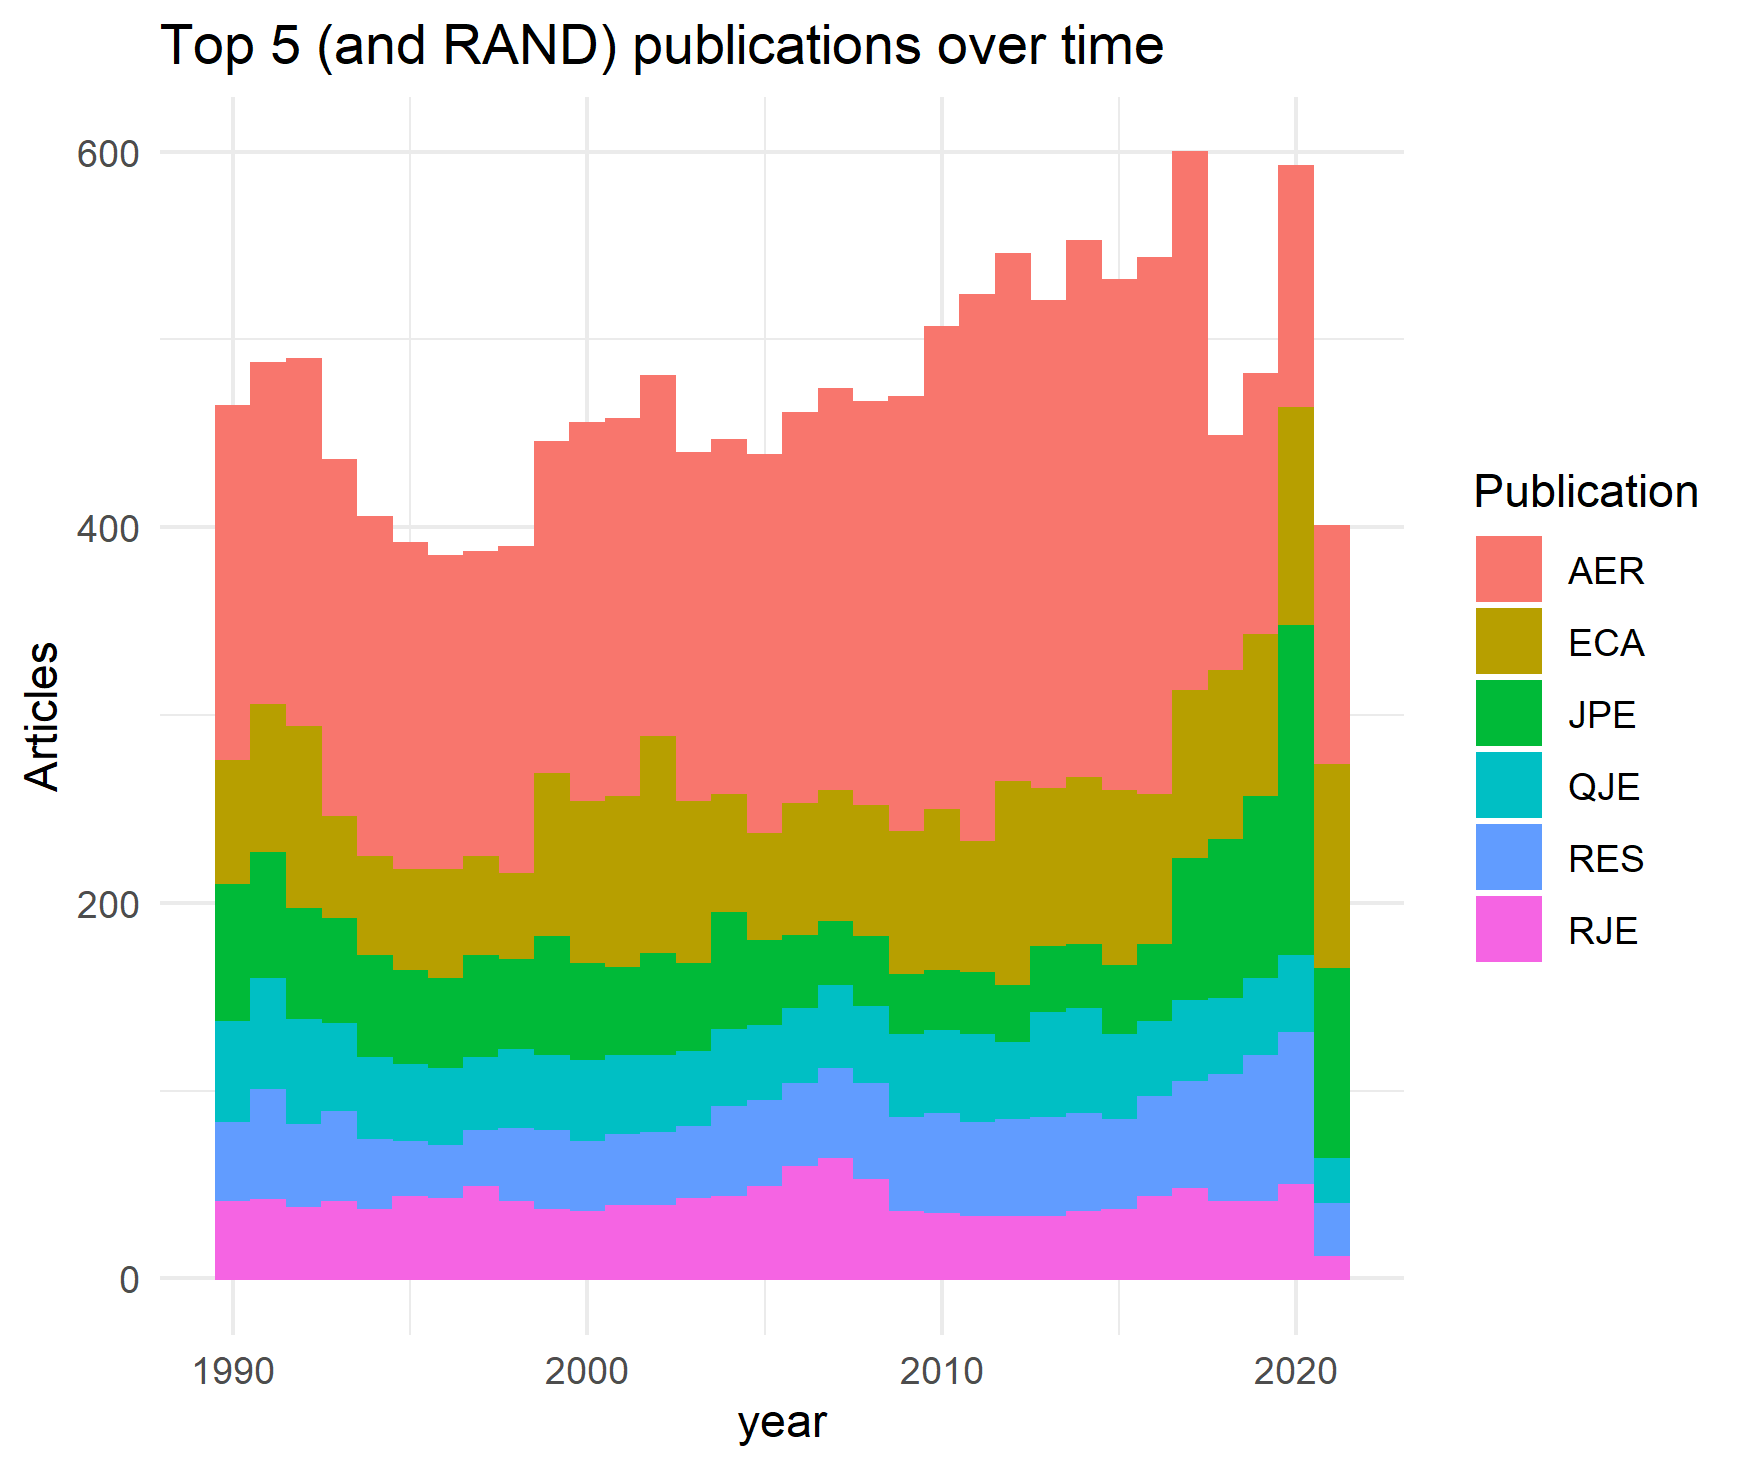
\includegraphics[width=\textwidth]{top_5_over_time_col.png}
        \caption{By count}
    \end{subfigure}
    \hfill
    \begin{subfigure}[h]{0.49\textwidth}
        \centering
        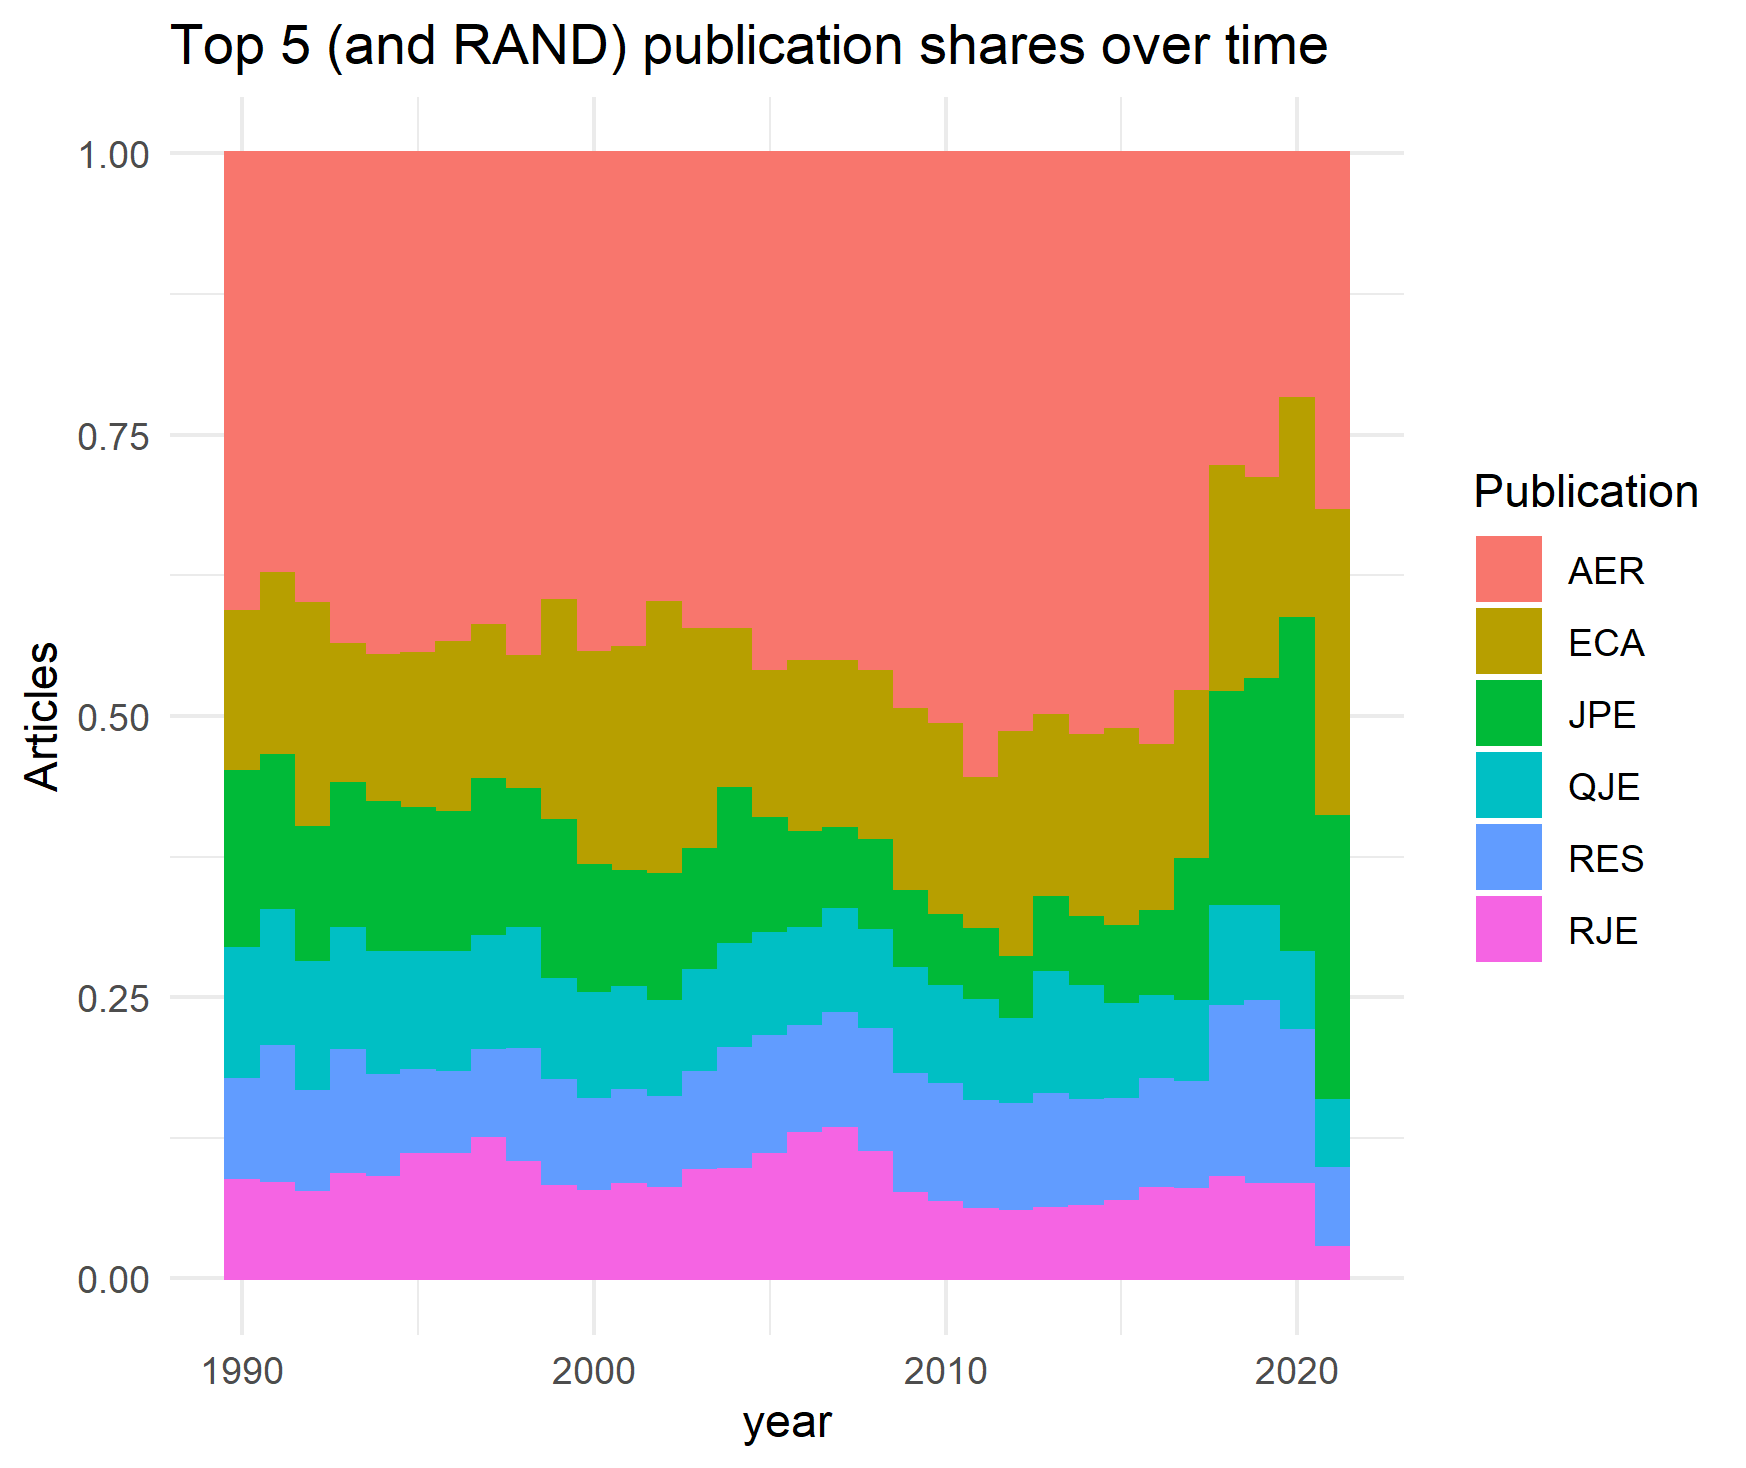
\includegraphics[width=\textwidth]{top_5_over_time_col_shares.png}
        \caption{By share}
    \end{subfigure}
    \begin{subfigure}[h]{\textwidth}
        \centering
        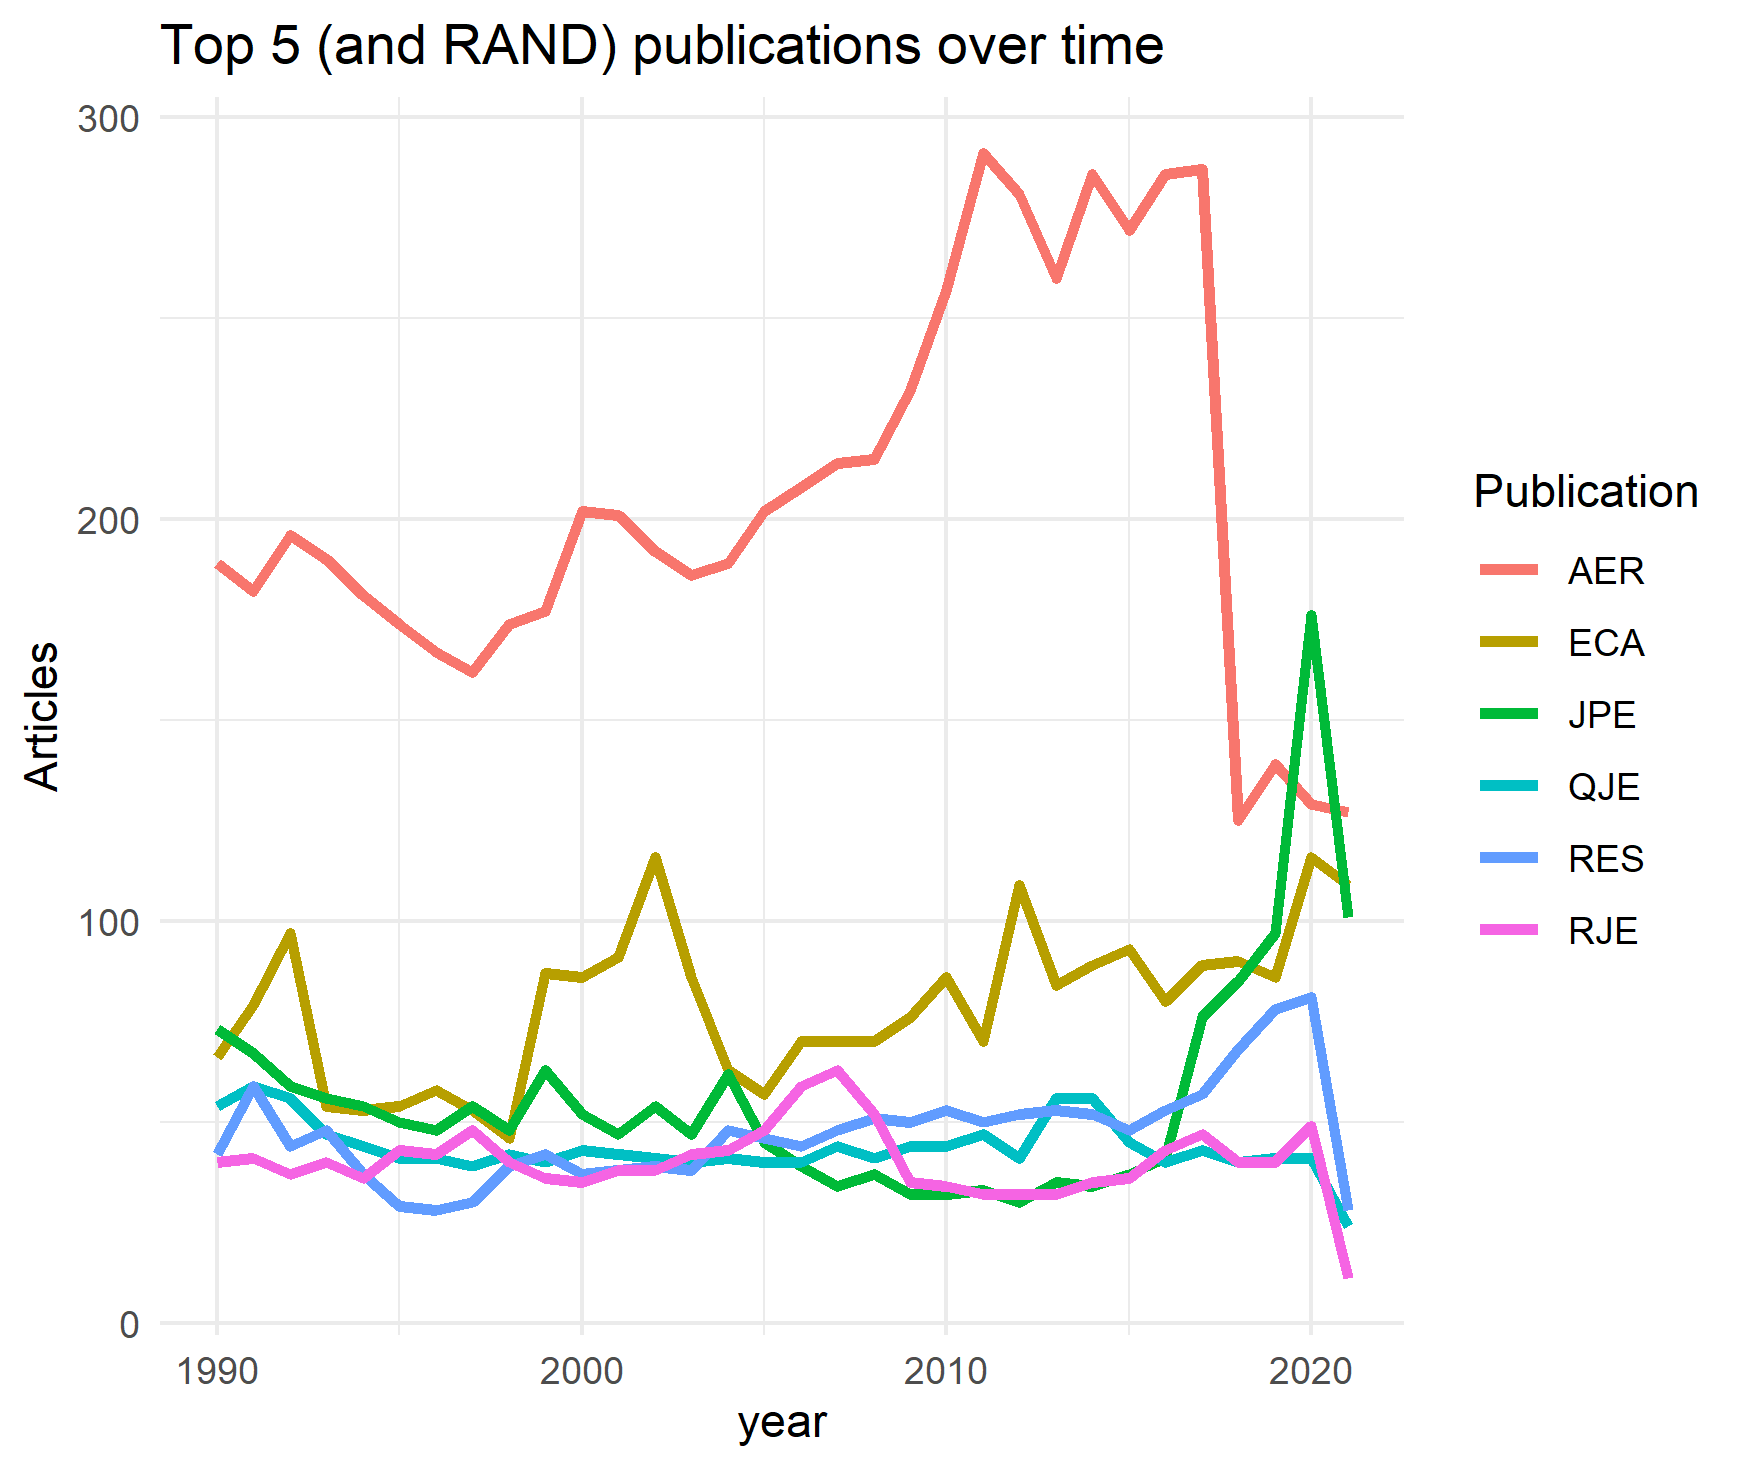
\includegraphics[width=0.5\textwidth]{top5_over_time.png}
        \caption{By count}
    \end{subfigure}
    \caption{Annual publications in the Top 5 (and RAND)}
\end{figure}

Though there has been some fluctuation over time, the Top 5 (and RAND) collectively published between 390 and 600 articles per year, with an average of 471 publications per year between 1990 and 2021.\footnote{Note that 2021 may bias this average downwards as not all articles may have yet been indexed by EconLit. Observations from 1990 are also potentially misleading as that year marked a major for the JEL code format (from a decimal-numeric system to an alpha-numeric system). Because not all articles use a uniform categorization format we omit observations from this year. Hereafter, we trim all data to consider only the period from 1991 to 2020.} See Appendix A for a full table of annual publication figures.\\

We also consider the composition of topics published in Top 5 over time.\footnote{In this instance we omit RAND because of its position as a field journal that is likely to have far less variation in topics published.} To assess this, we construct two measures of topics. First, we identify a ``predominant'' JEL code among those listed on a paper. For example, if a paper is published with five JEL codes --- C53, E43, F31, F37, and G15 for instance --- because there are two codes that begin with ``F'', we identify the paper as an ``International Economics'' paper. Ties are resolved by random number generator. Using this measure, Figure 2 plots the distribution of topics over time.


\begin{figure}[!ht]
    \centering
    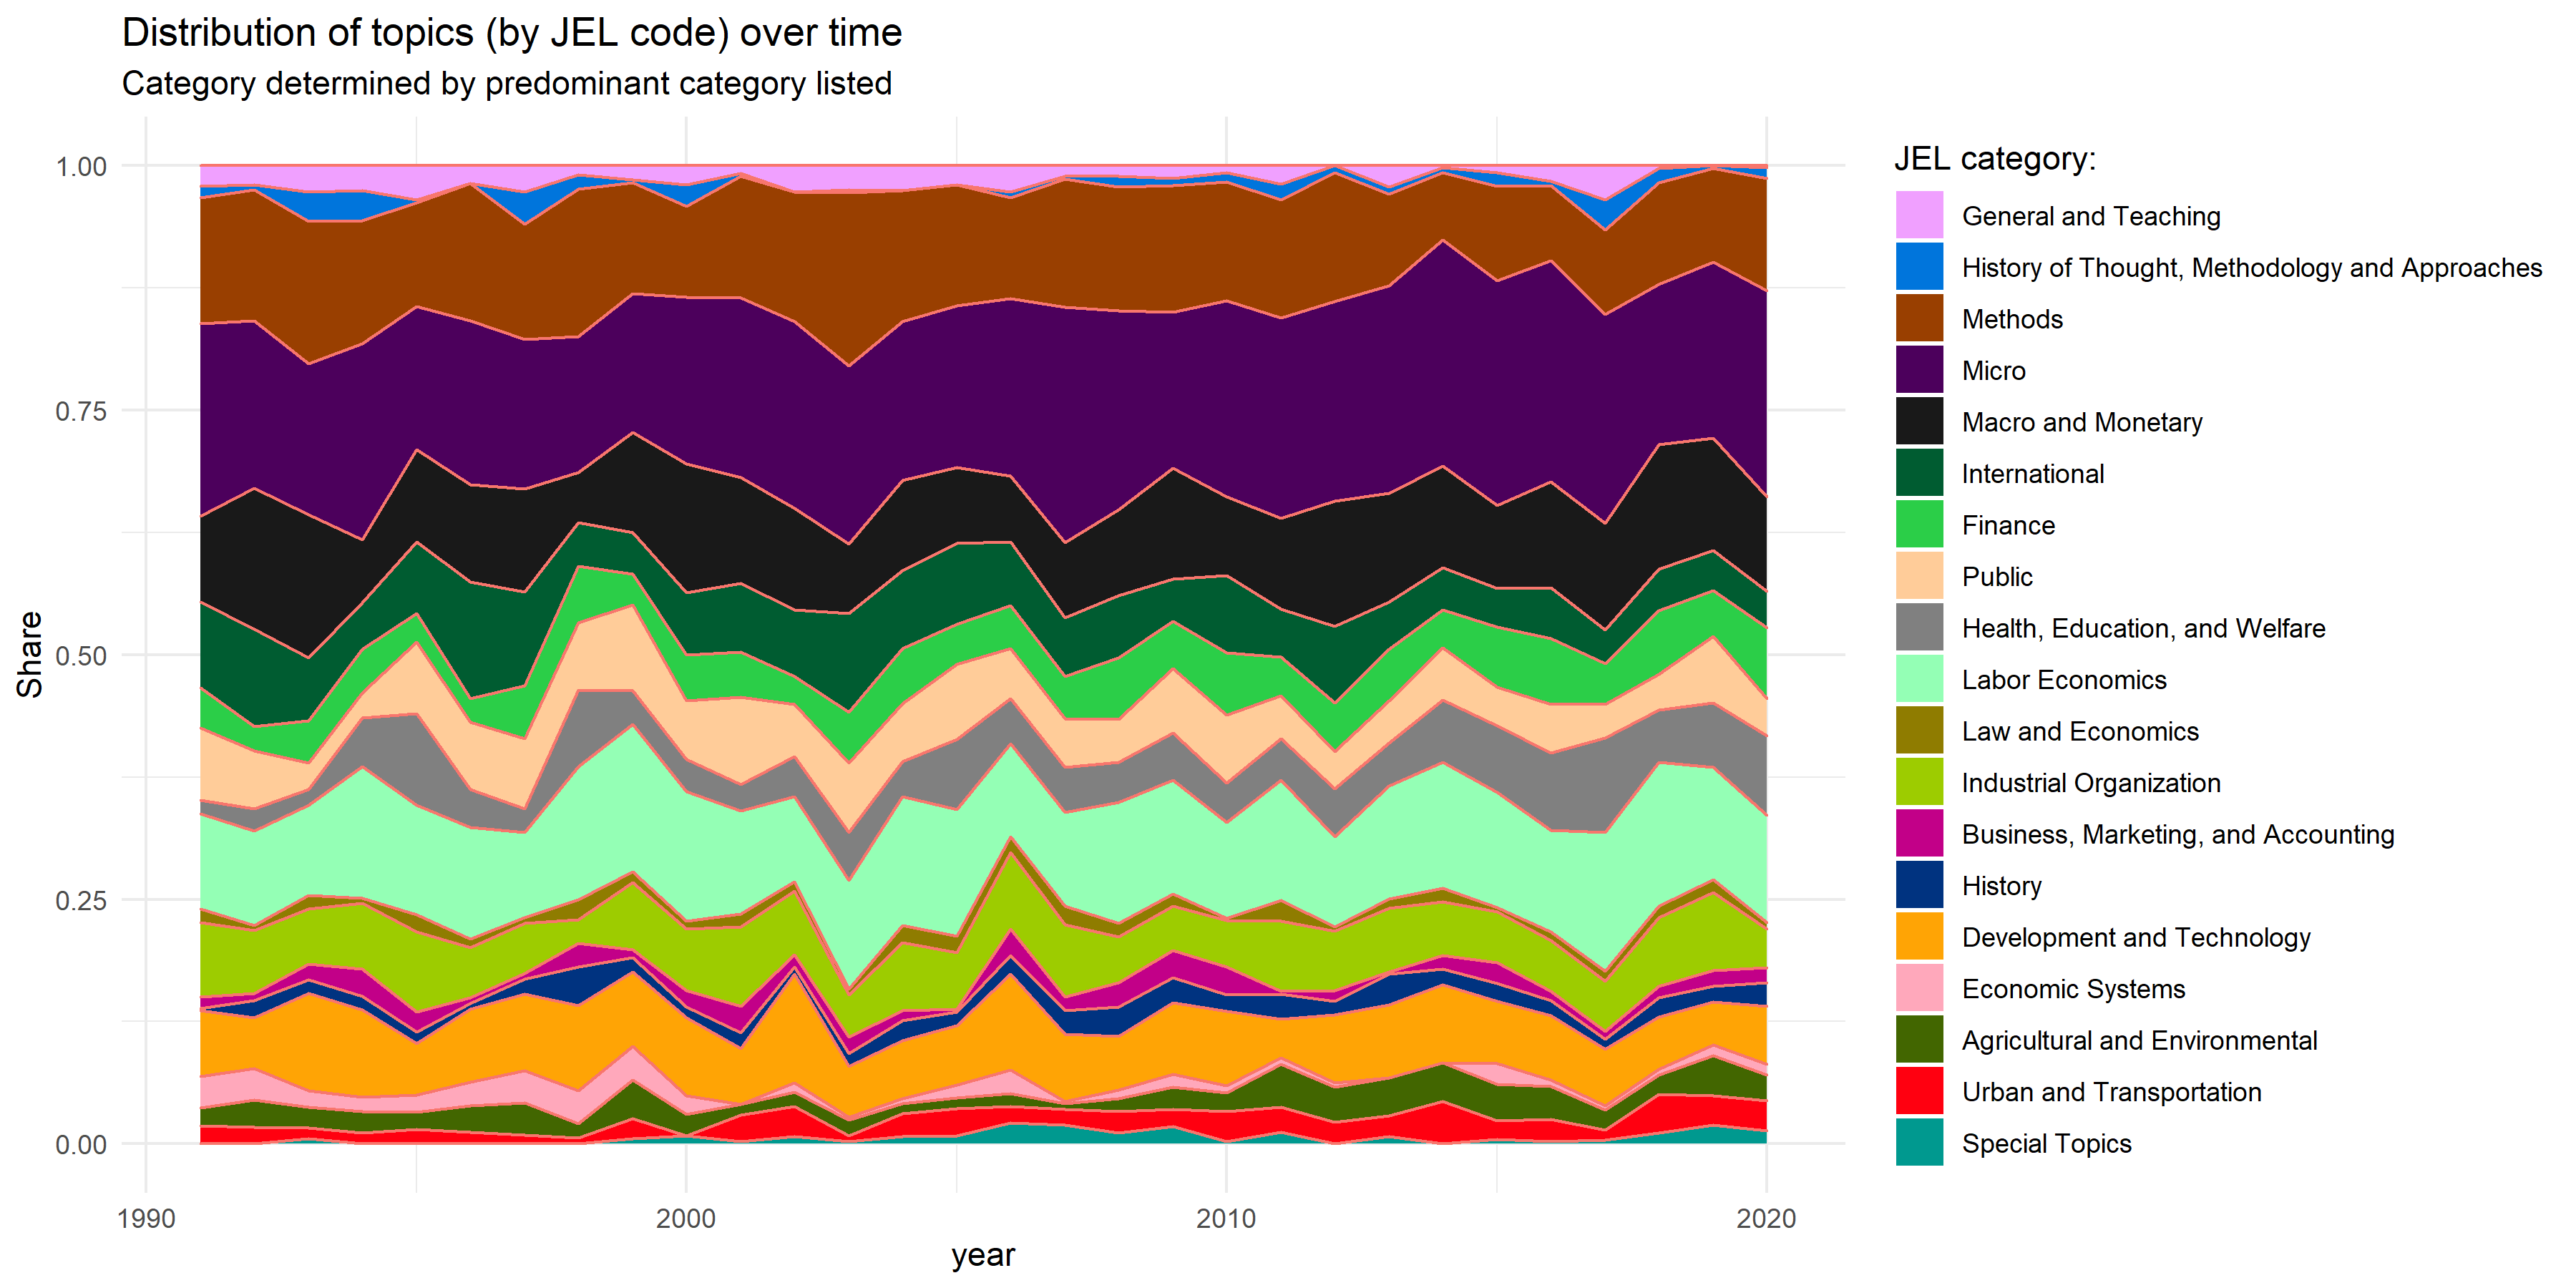
\includegraphics[width=\textwidth]{jel_predom_normalized.png}
    \caption{Topics in the Top 5 journals over time.}
\end{figure}




We also use a weighted-frequency approach to identify trends in topic publication over time. For this measure, using the same codes as above, such a paper would receive four JEL categorizations --- ``C,'' ``E,'' ``F,'' and ``G'' each with weights commensurate with their within-paper frequency. That is, ``F'' would receive 40\% weight, and the remaining codes would each receive 20\% weights. These weights are then aggregated over each journal for each year. The results are presented below in Figure 3. When using this measure, we hereafter continue to use the terms ``articles,'' or ``publications'' for purposes of consistency. However, this measure more precisely refers to the number or share of particular JEL codes relative to all JEL codes published in the Top 5/the journal of interest.

\begin{figure}[!ht]
    \centering
    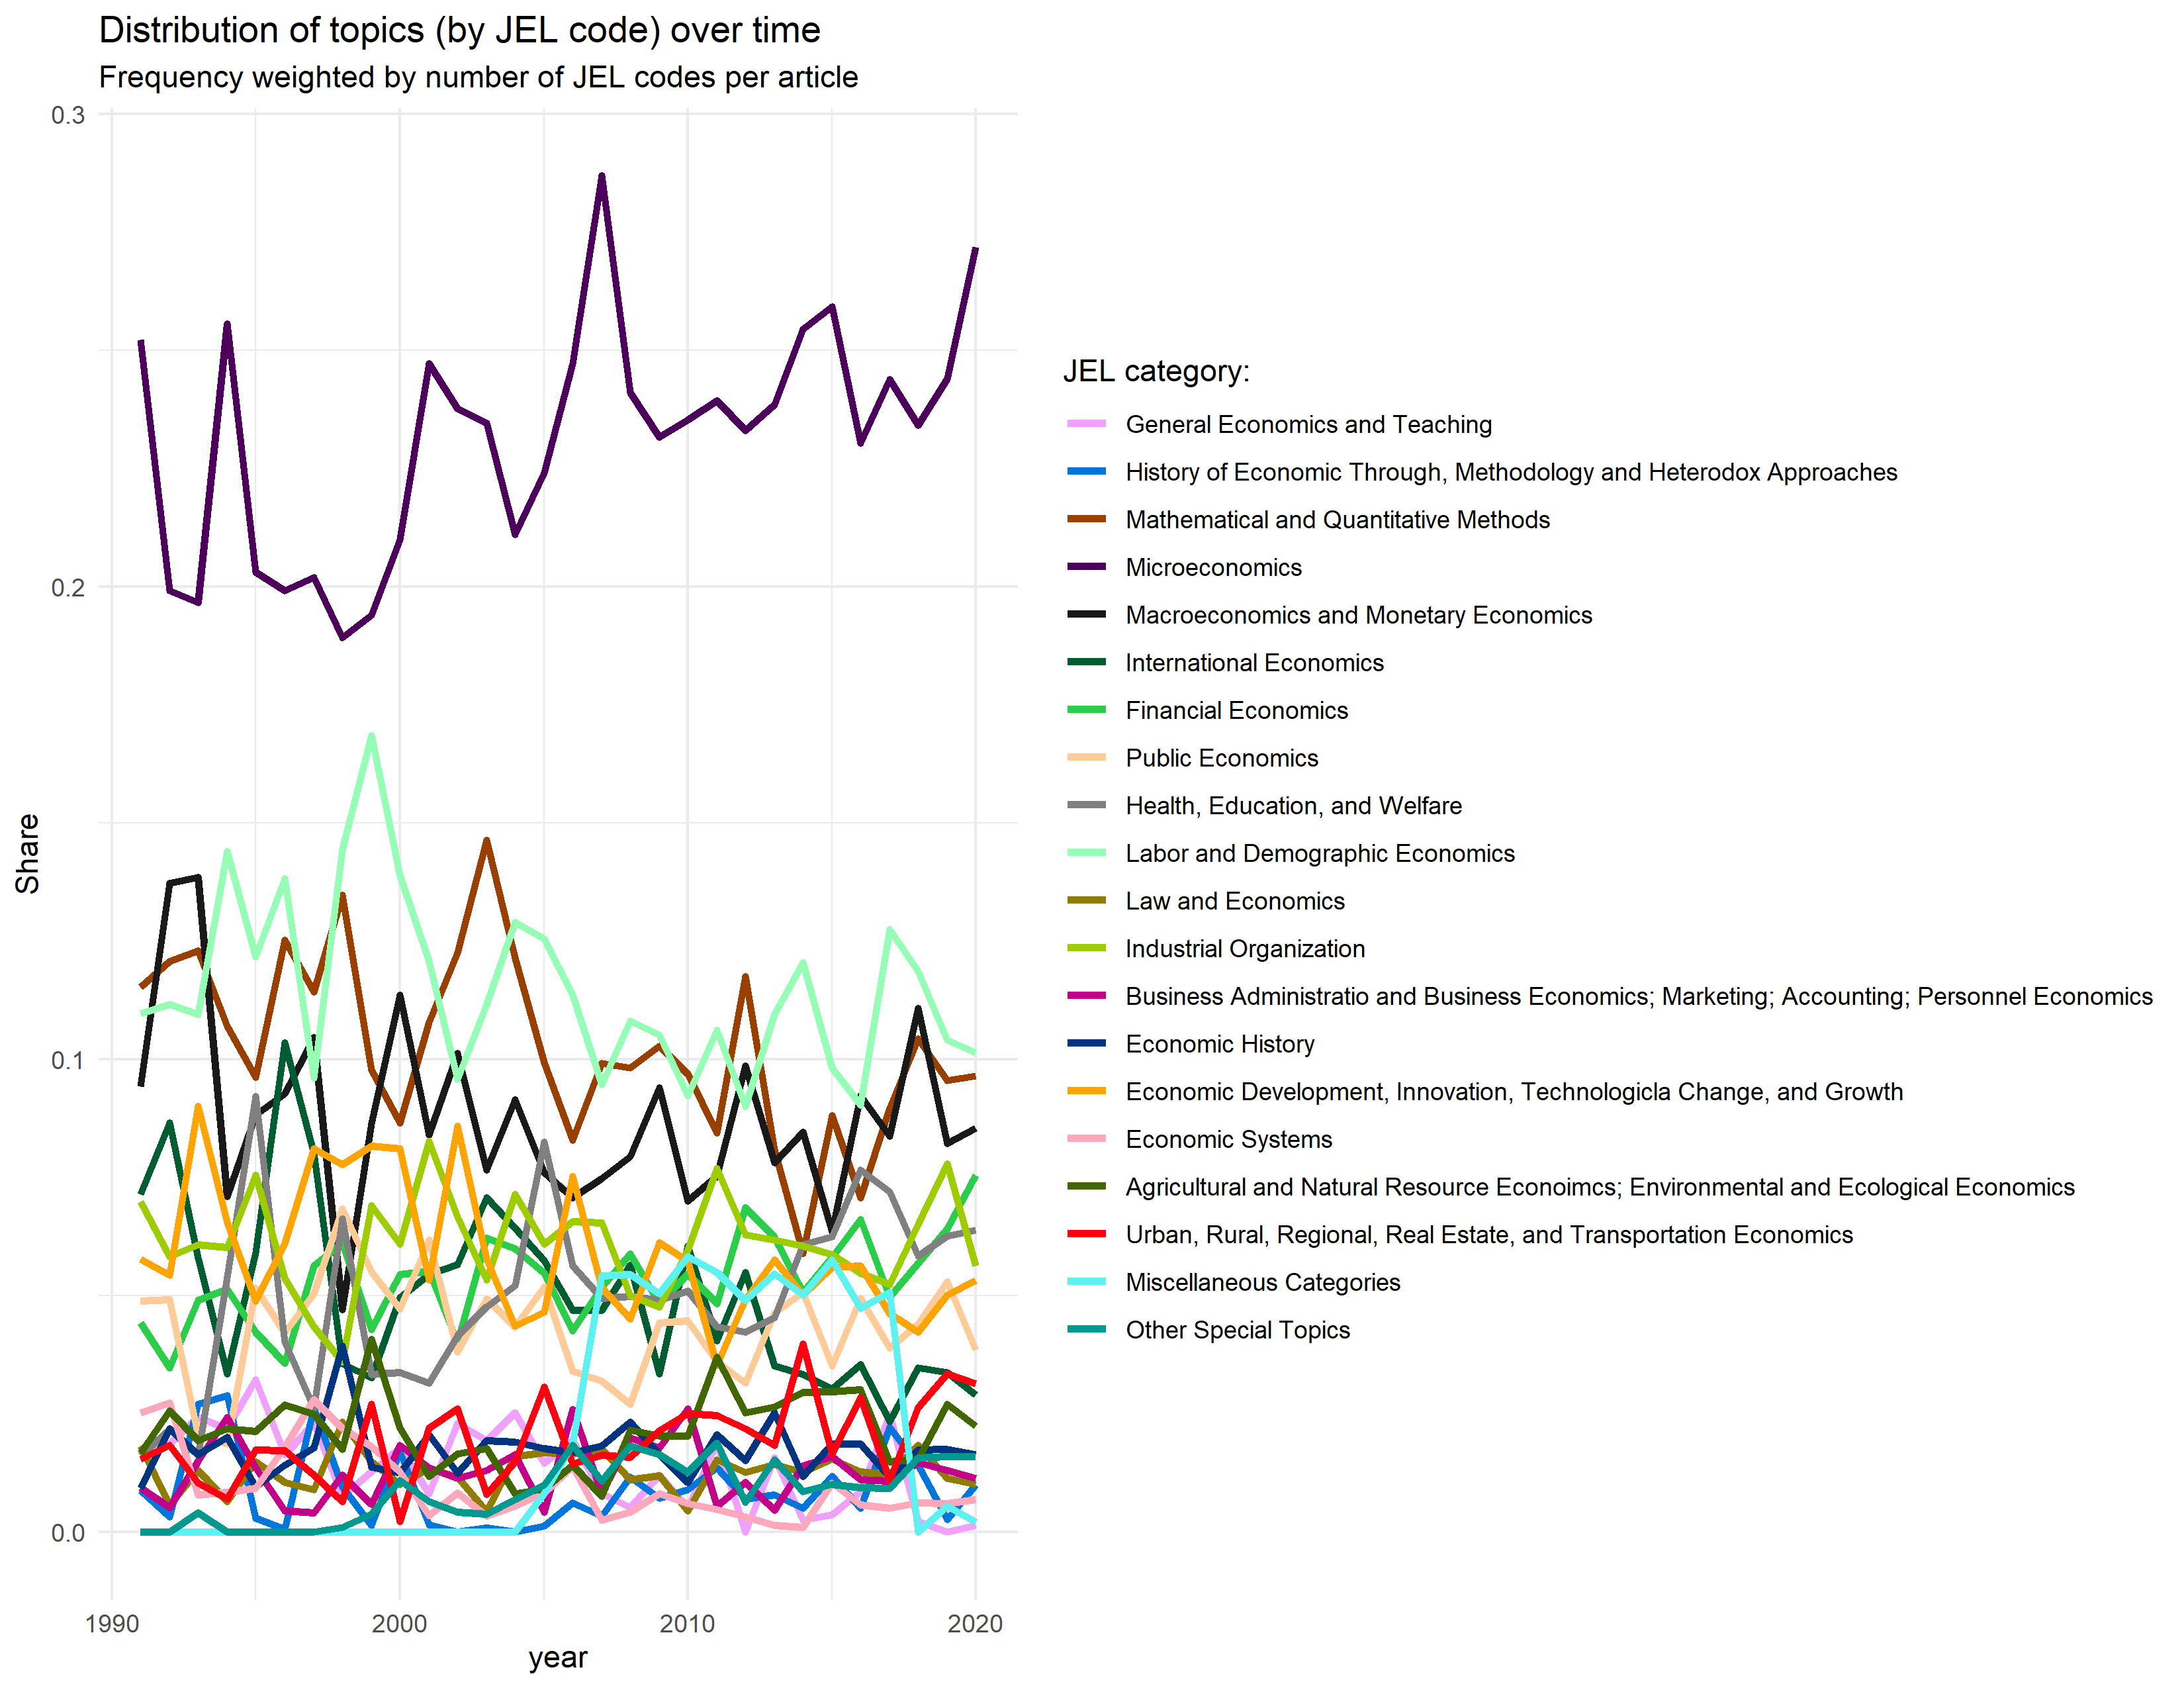
\includegraphics[width=\textwidth]{jel_weighted_normalized_line.png}
    \caption{Topics in the Top 5 journals over time. N.B.: The vertical-axis has been broken twice in order to improve legibility by creating more space between series.}    
\end{figure}

Throughout, the time series, papers in ``Microeconomics'' (D) have taken up an outsized share of Top 5 publications. There are some other topics that constitute a disproportionate share of publications, such as ``Labor Economics'' (J) and ``Mathematical and Quantitative Methods'' (CXX), but both such categories are on the order of half a magnitude smaller than microeconomics. In this time sample, ``Industrial Organization'' (L) papers constitute between 3\% (in 1998) and 8\% (in 2001) of Top 5 publications.\\

We then use the same measure to consider how topics are represented in each of the Top 5 journals. In Figure 4 below, similar trends as above are identifiable. Microeconomics is well represented in all of the Top 5 journals (though less so in the AER and QJE), as is Labor (with the exception of \textit{Econometrica}). \textit{Econometrica} stands out as being the least topic-diverse of the Top 5 journals, with its publications being much more focussed on quantitative methods topics and microeconomics than the other journals' more general-interest profiles. As above, it is hard to identify clear trends in topic popularity over time. That is, \textit{prima facie}, Industrial Organization appears to constitute a small part of the Top 5 literature, but not particularly so relative to other topics.\footnote{For an ordinal ranking of topics in each of the Top 5 journals for selected years, see Appendix A Table 2.}


\begin{figure}[h]
    \centering
    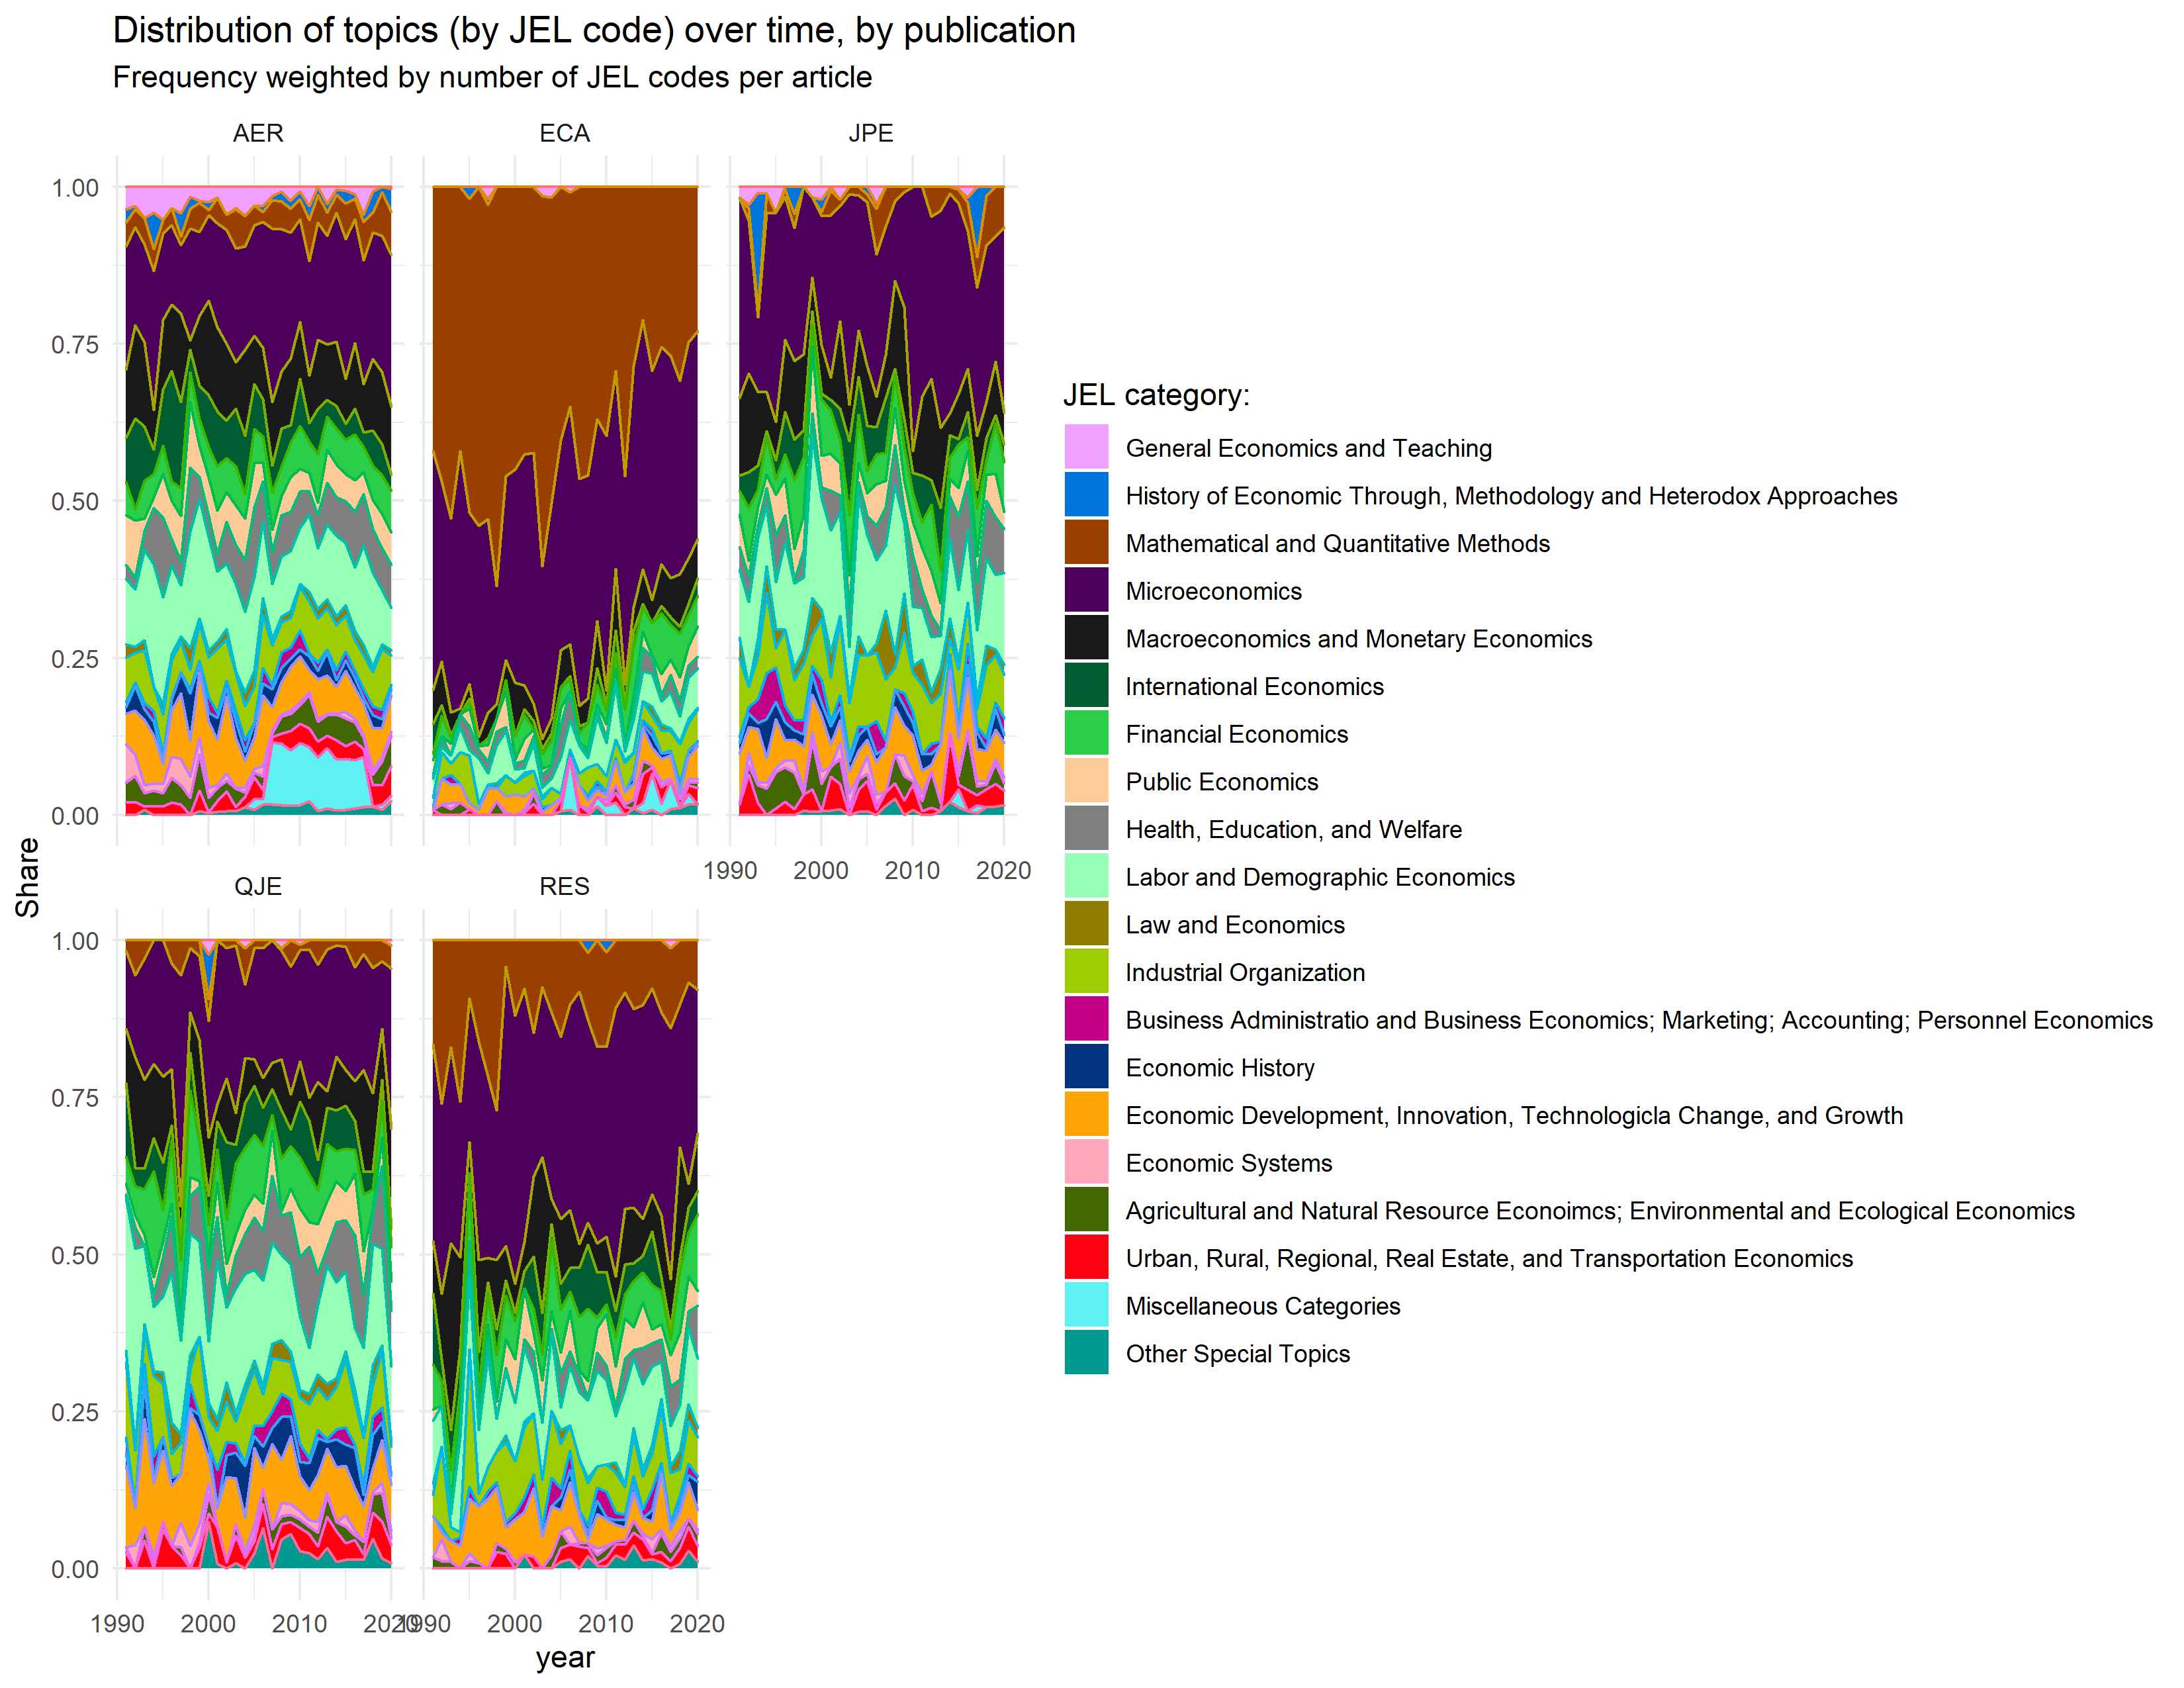
\includegraphics[width=\textwidth]{jel_weighted_normalized_by_journal.png}
    \caption{Topics in the Top 5 over time}
\end{figure}



\section{The Role of Industrial Organization}
We then consider how Industrial Organization (IO) papers have featured in the Top 5 and RAND over time. We consider a paper to be an ``IO'' publication if the article's associated Journal of Economic Literature (JEL) codes contains \textit{at least} one code that begins with ``L,'' hereafter regularly referred to as LXX. (JEL codes since 1990 have been a letter followed by two numbers, each indicating a greater degree of topic-specificity.) There are other JEL codes which could ostensibly be considered IO-related. These include K21 (Antitrust law), D4 (Market structure, pricing, and design), O3 (Innovation; research and development; technological change; intellectual property rights), and G34 (Mergers; acquisitions; restructuring; corporate governance). However, these are omitted at first to make comparisons across various topics/groups easier. Using this methodology, we identify 2,380 IO-related articles across the Top 5 (and RAND) between 1991 and 2020.\\

\begin{figure}[!ht]
    \begin{subfigure}[h]{0.49\textwidth}
        \centering
        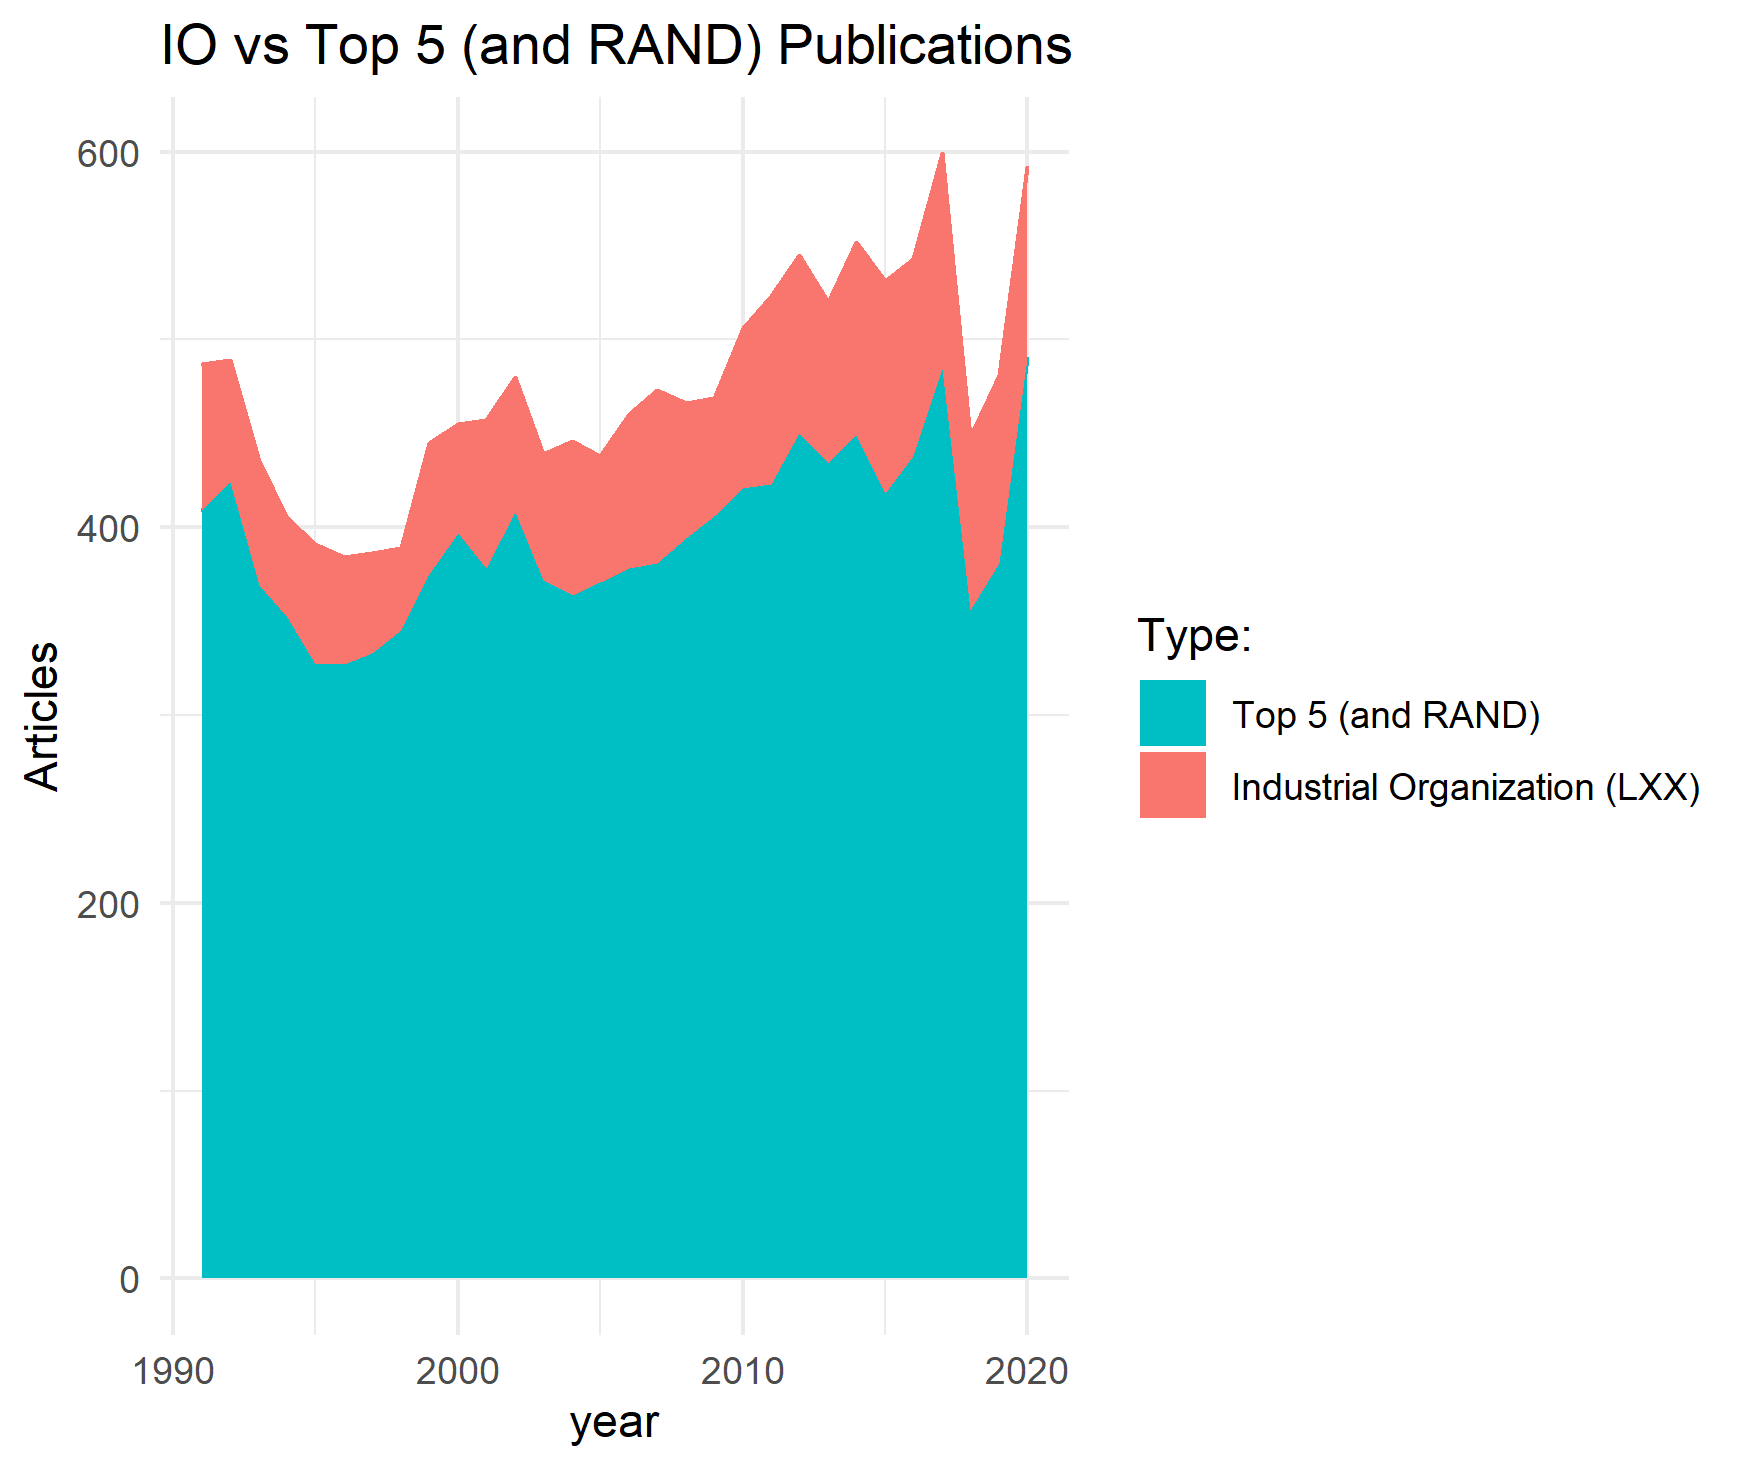
\includegraphics[width=\textwidth]{LXX-code-share-area.png}
        \caption{By count}
    \end{subfigure}
    \hfill
    \begin{subfigure}[h]{0.49\textwidth}
        \centering
        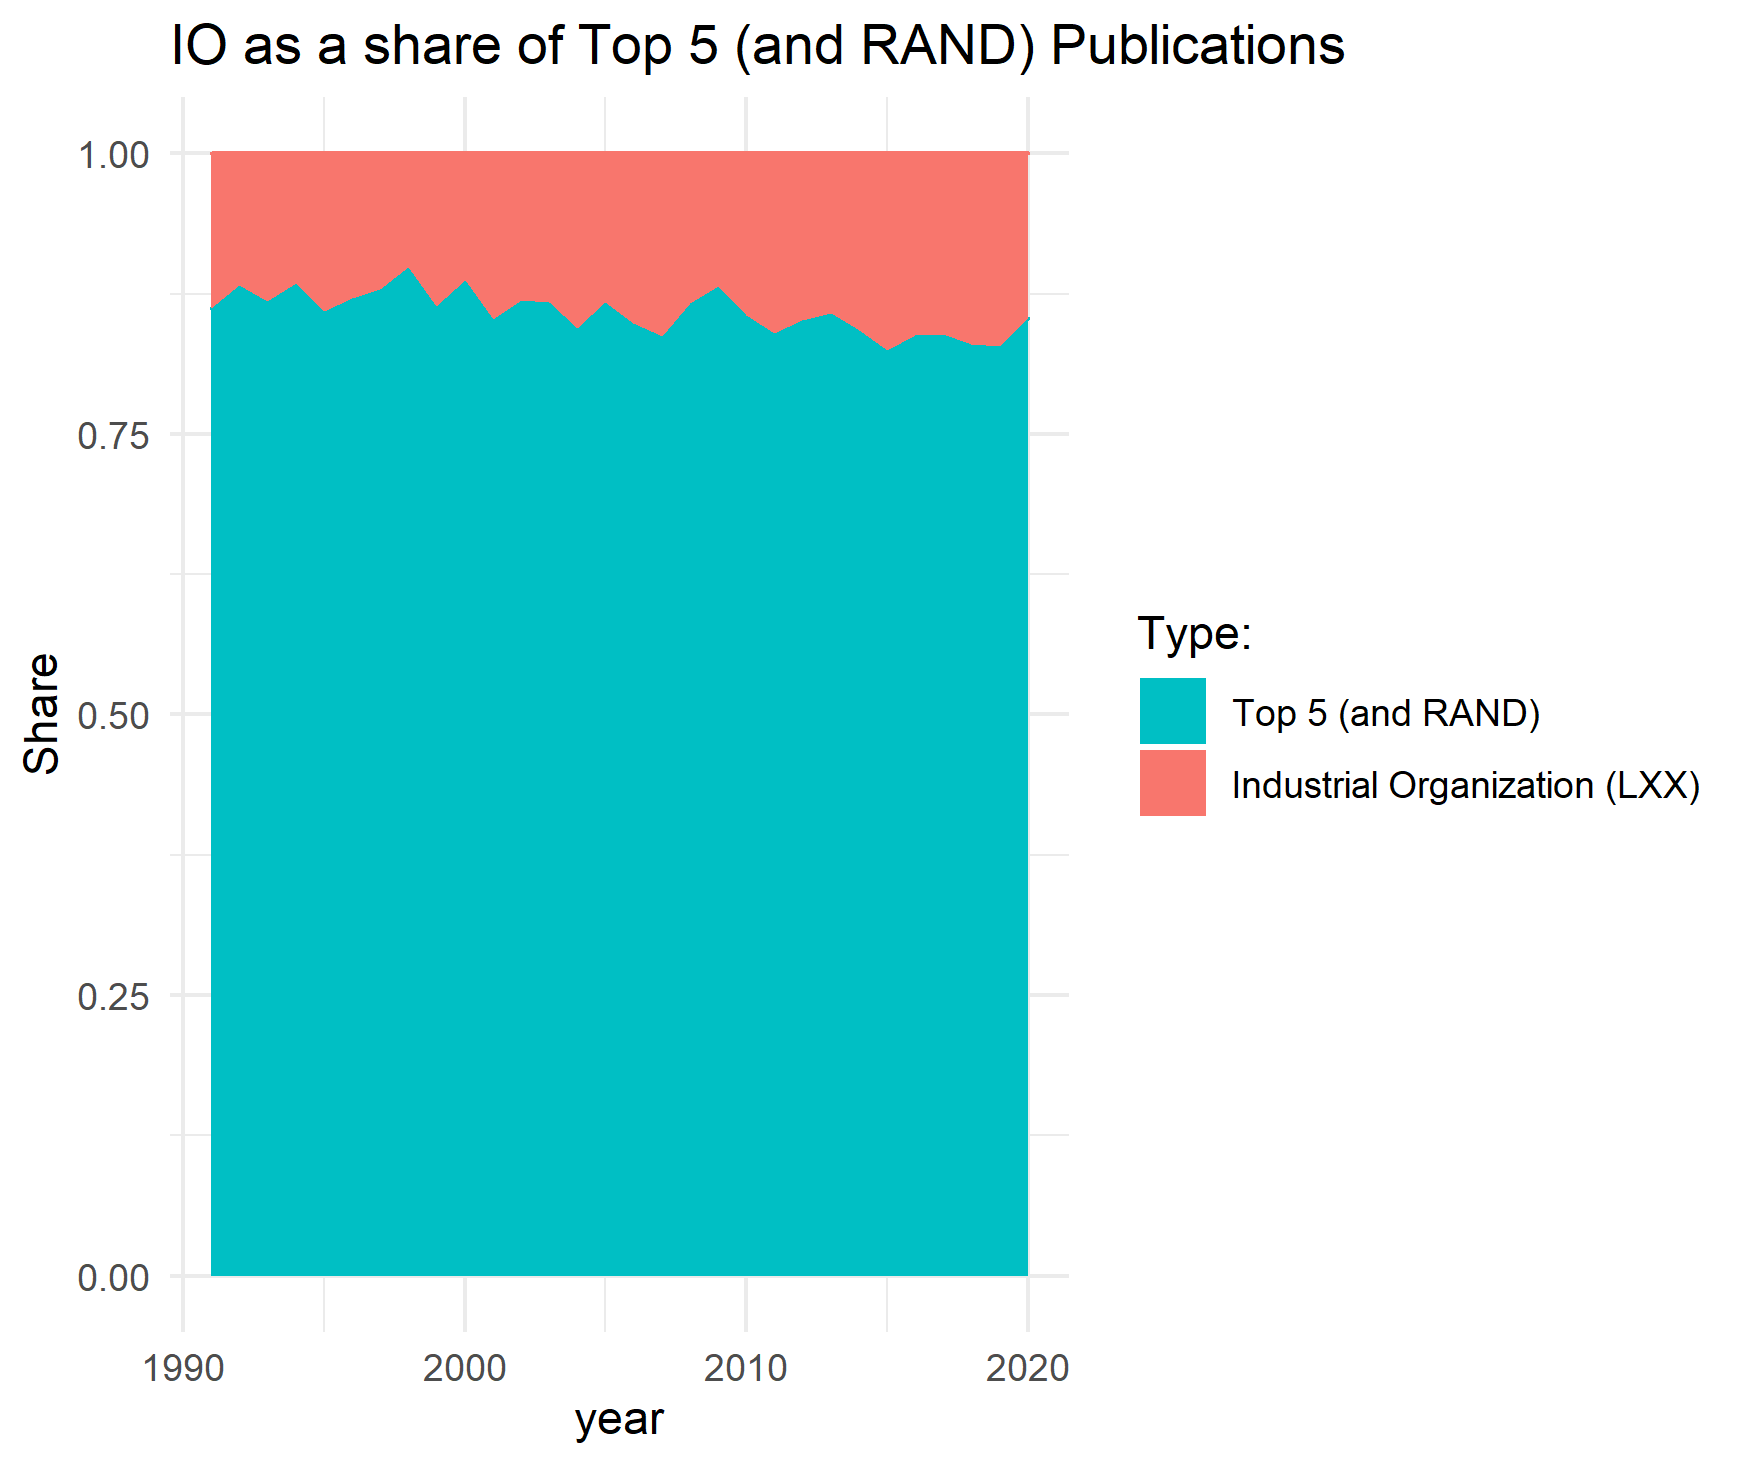
\includegraphics[width=\textwidth]{LXX-code-share-area-normalized.png}
        \caption{By share}
    \end{subfigure}
    \caption{Industrial Organization in the Top 5 (and RAND)}
\end{figure}

During the the period from 1990 to 2020, IO papers have made up, on average, approximately 16\% of articles published in the Top 5 (and RAND). This share has grown steadily over time, with the greatest share of such articles having been published in 2020 (20.8\%).\footnote{See Table 2 in Appendix B for a full table of annual IO share figures.} This pattern, however, is not agnostic pf journal. That is, the AER and QJE, publish lots of IO papers relative to, for example, \textit{Econometrica}. Additionally, as is to be expected of a field journal, \textit{RAND} regularly sees almost 40\% its publications mention at least one LXX JEL code.\footnote{For an annual breakdown of by-journal IO shares, please see Appendix B Table 4.} \\

Additionally, the inclusion of RAND may be misleading. As noted above, when excluding RAND, IO papers make up only between 3\% and 8\% of articles published in the Top 5 journals. Those shares appear to be in conflict with those plots presented below in Figure 5 (b), which, for many of the publications of interest, present significantly larger shares. However, recall that Figures 3 and 4 above presented the article-level \textit{weighted} frequency of JEL codes, whereas Figure 6 the \textit{absolute} frequency of LXX JEL codes. That is, the seemingly contradictory results of these two figures are reconcilable in the case that IO-related articles are frequently published with lots of other JEL codes also listed on the those articles (thereby reducing the weight afforded the LXX code in Figure 3).

\begin{figure}[!ht]
    \begin{subfigure}[h]{0.49\textwidth}
        \centering
        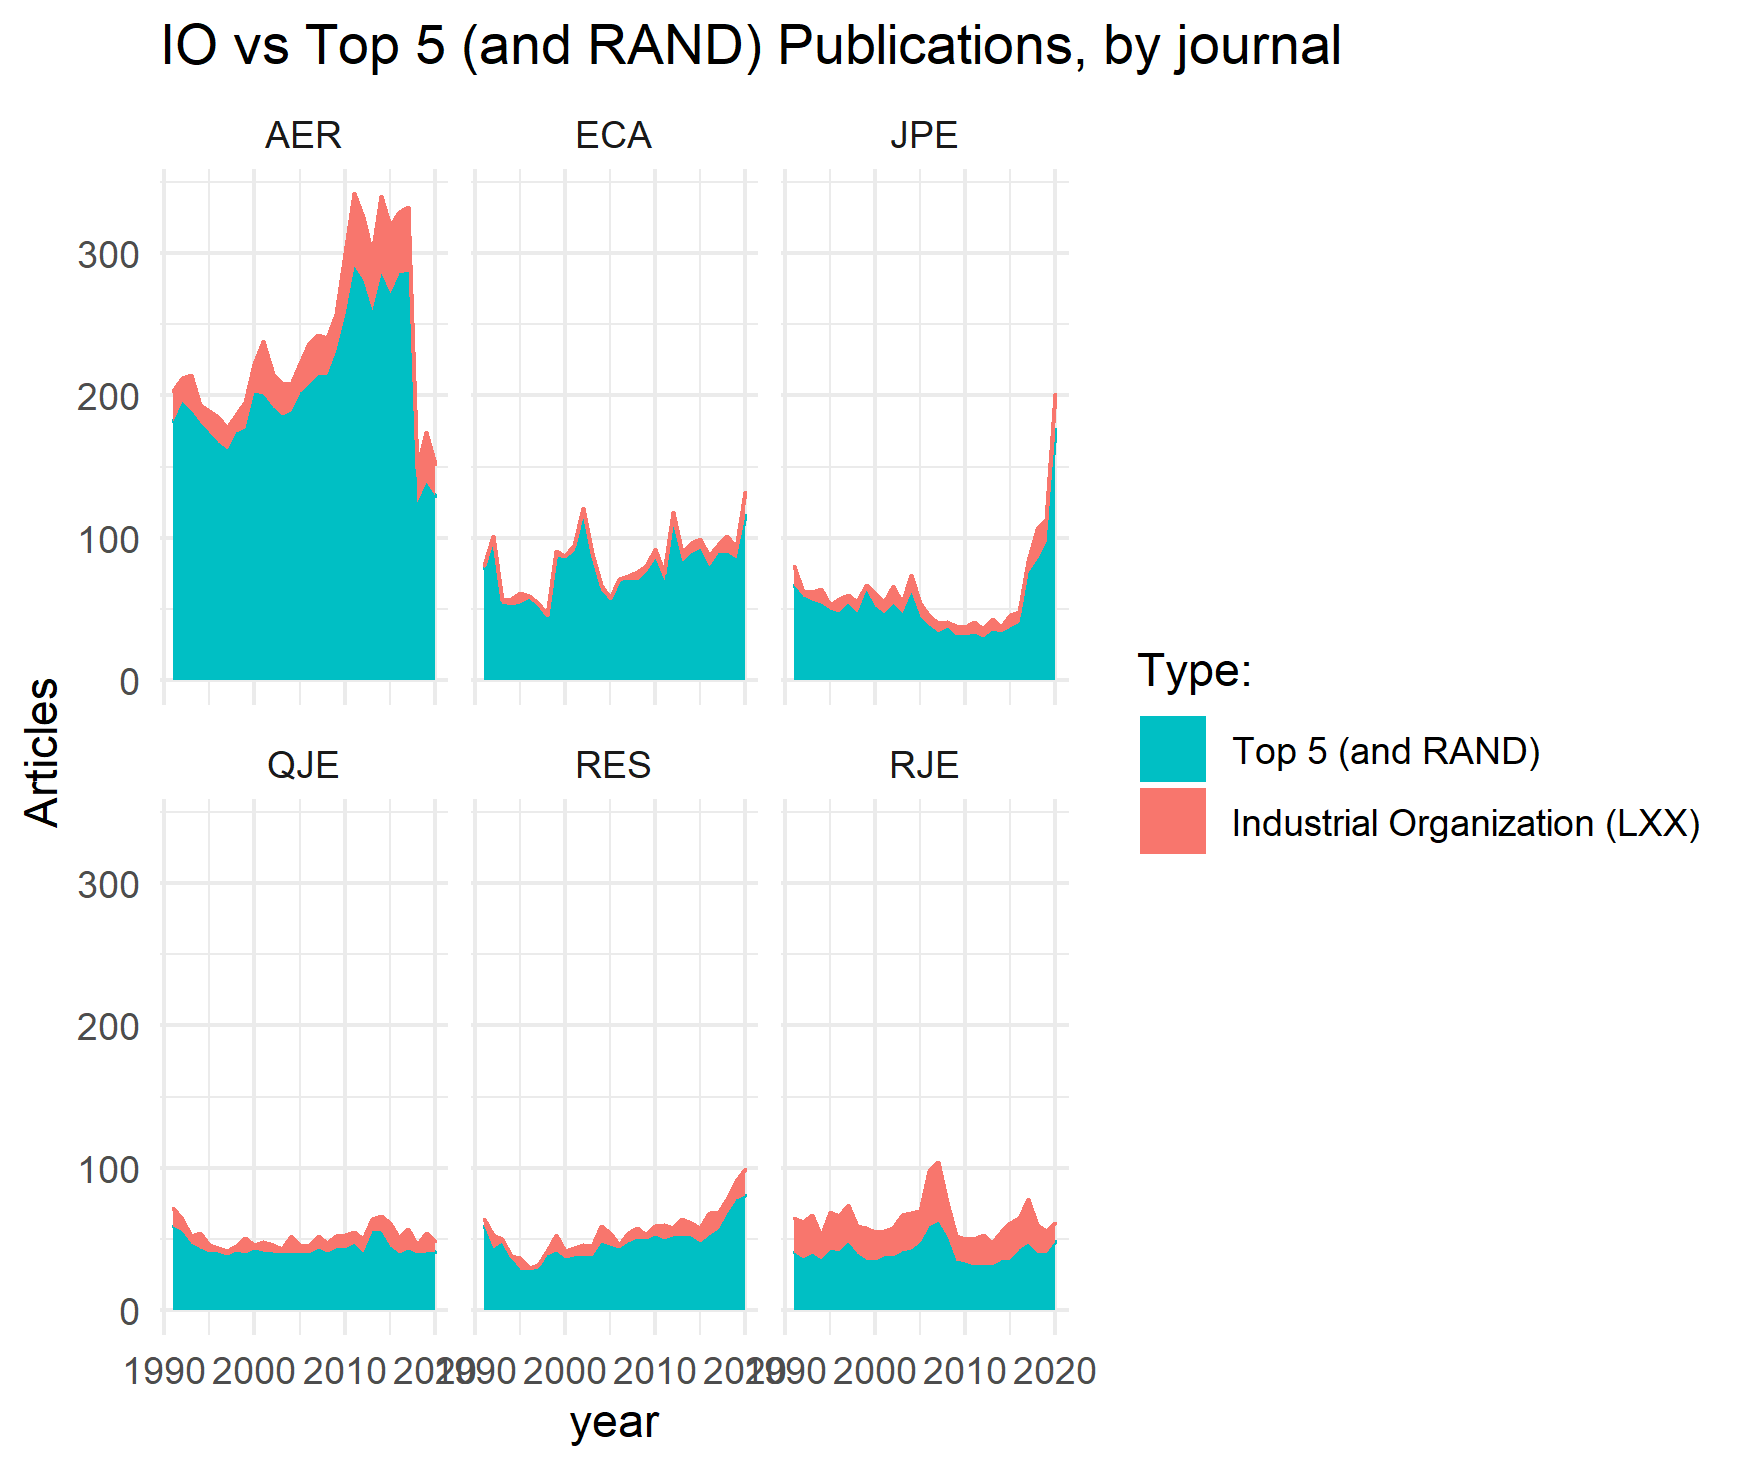
\includegraphics[width=\textwidth]{LXX-code-share-area-by-journal.png}
        \caption{By count}
    \end{subfigure}
    \hfill
    \begin{subfigure}[h]{0.49\textwidth}
        \centering
        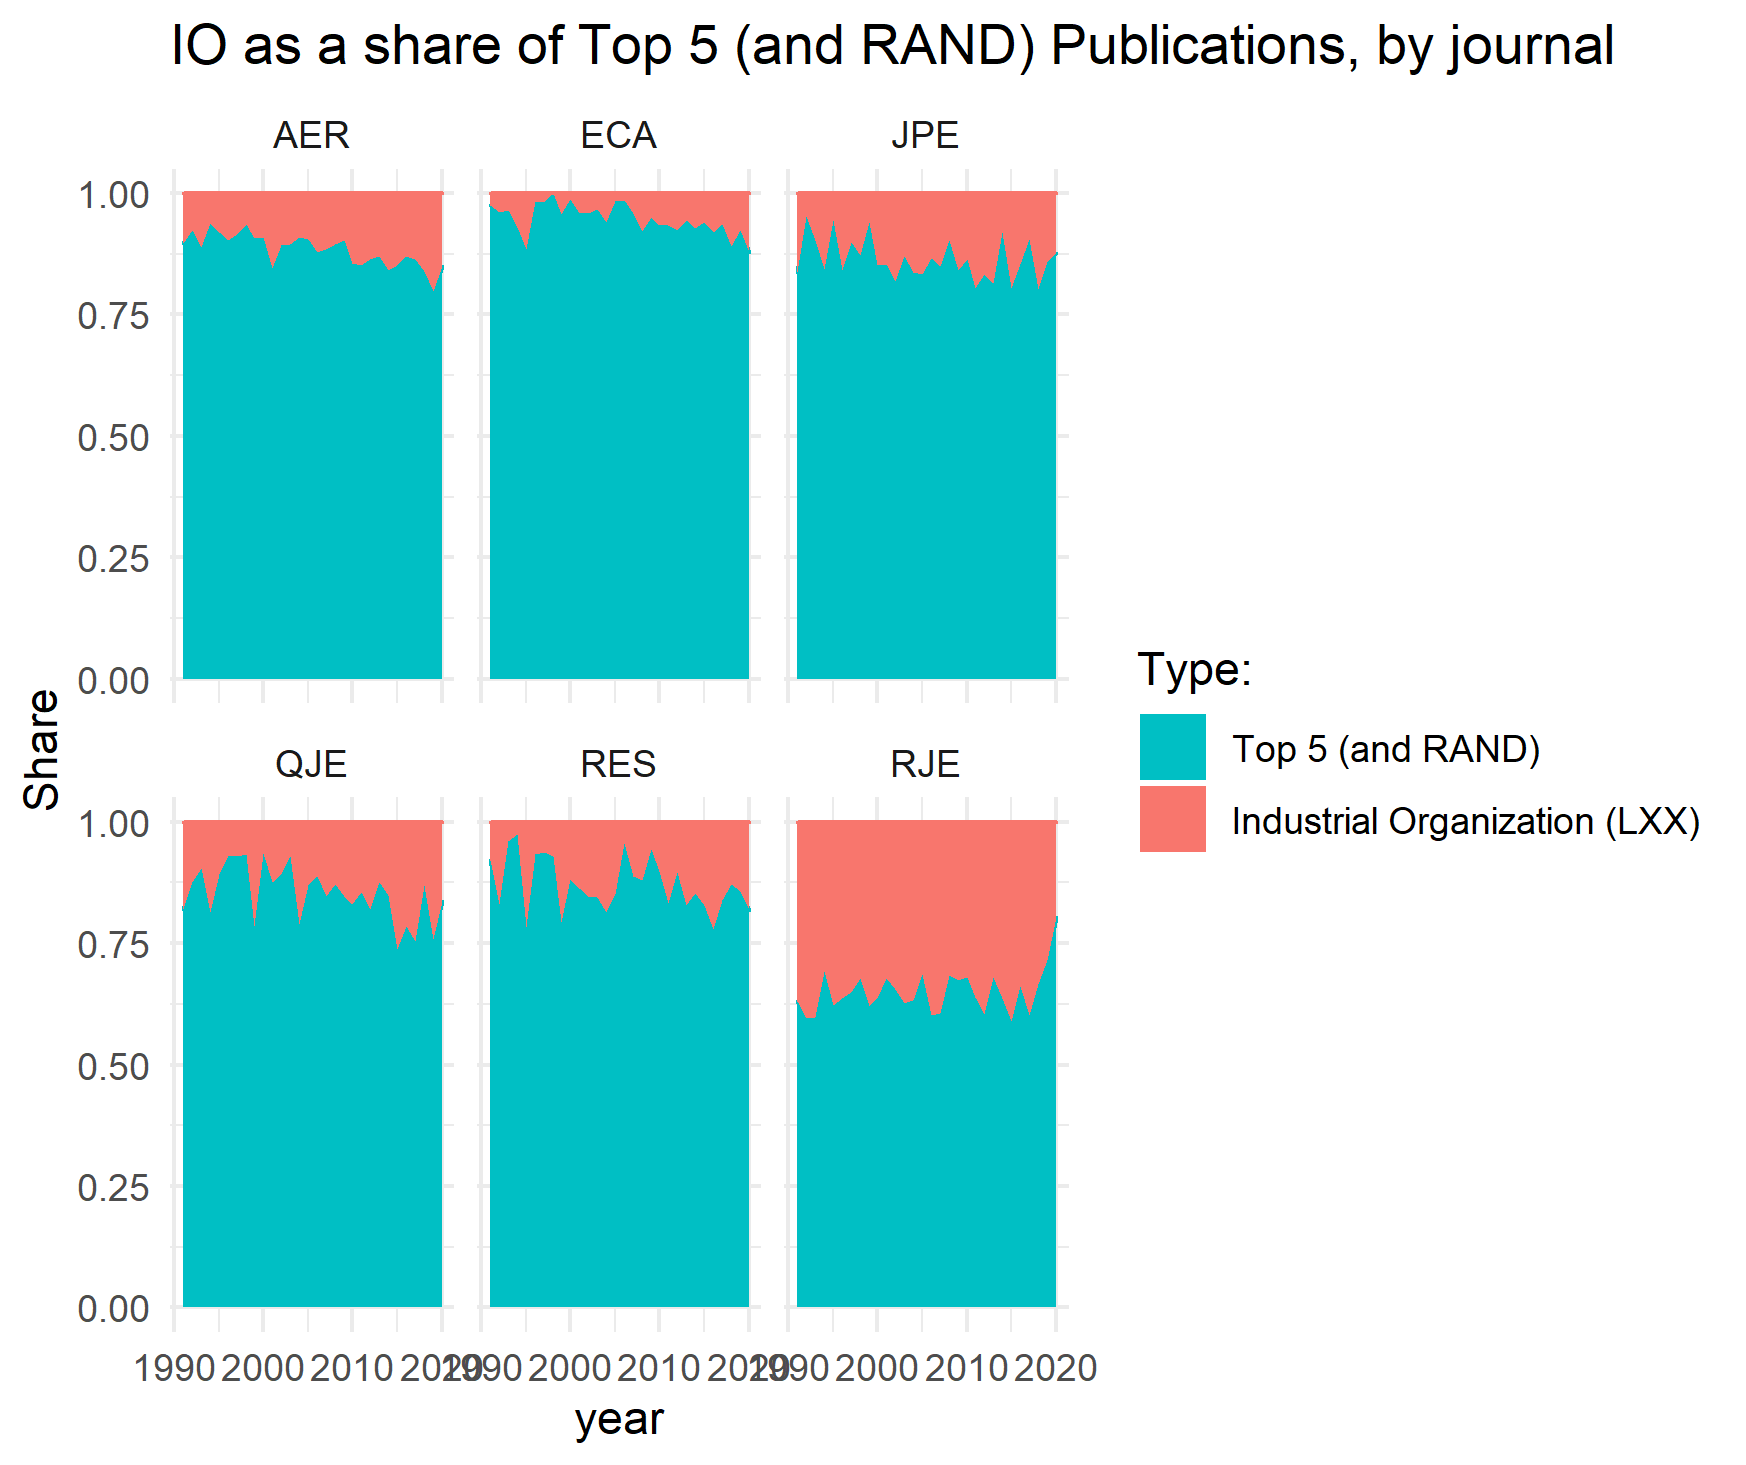
\includegraphics[width=\textwidth]{LXX-code-share-area-normalized-by-journal.png}
        \caption{By share}
    \end{subfigure}
    \caption{Industrial Organization in the Top 5 (and RAND), by journal}
\end{figure}

\newpage

\section{The Role of Anti-Trust}
Even within ``L'' Industrial Organization category, there are 10 classes of JEL codes that refer to topics from ``Market structure, firm strategy and market performance'' (L1) to ``Industry studies: transportation and utilities'' (L9). We are particularly interested in the papers published in the Top 5 (and RAND) that bear at least one L4 code, indicating that the paper pertains to ``Antitrust issues and policies.''\\

\begin{figure}[!ht]
    \begin{subfigure}[h]{0.49\textwidth}
        \centering
        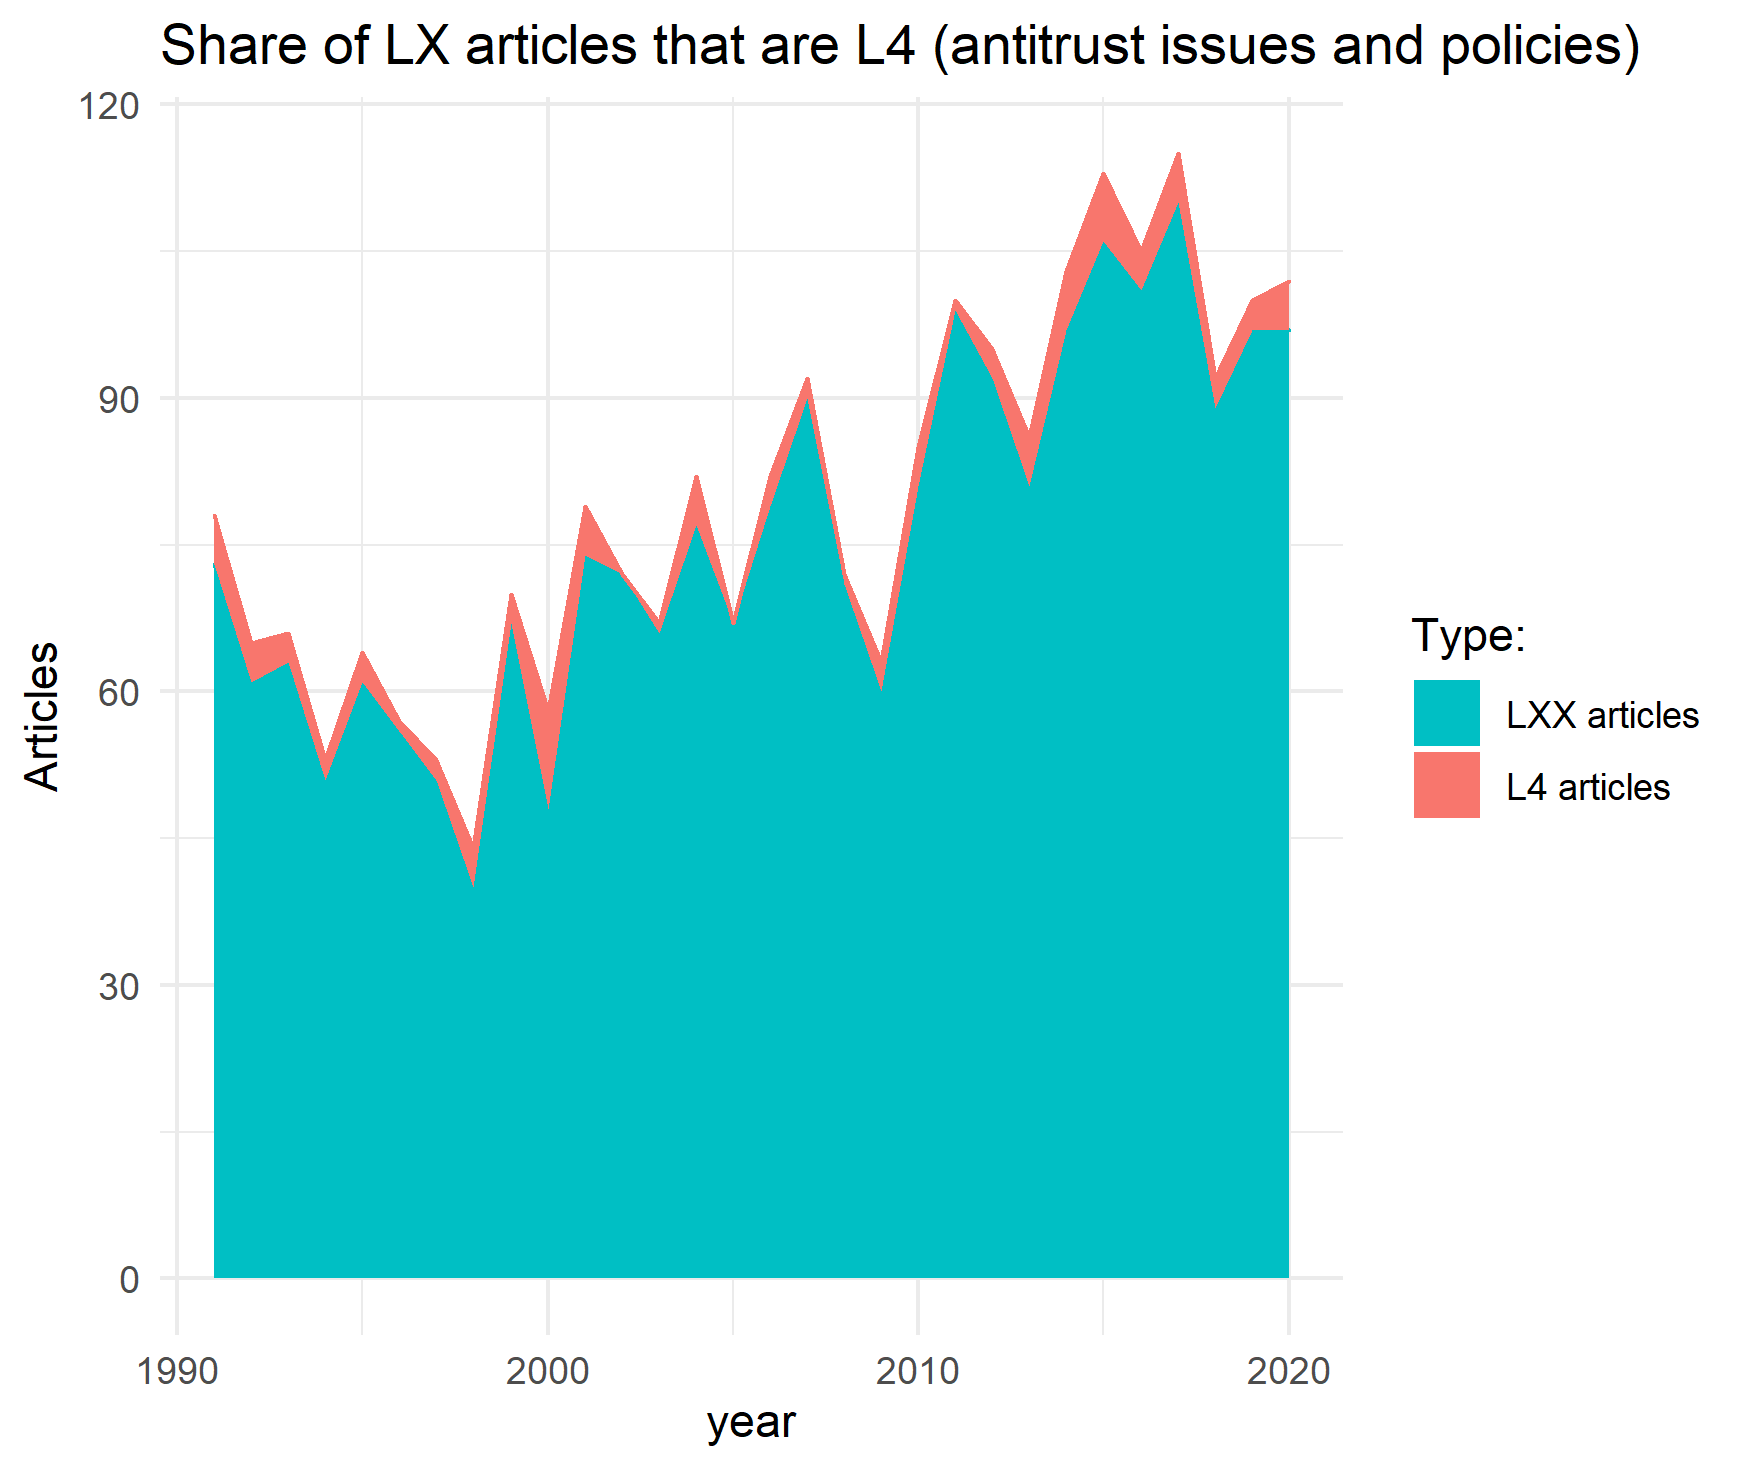
\includegraphics[width=\textwidth]{L4-vs-LXX.png}
        \caption{By count}
    \end{subfigure}
    \hfill
    \begin{subfigure}[h]{0.49\textwidth}
        \centering
        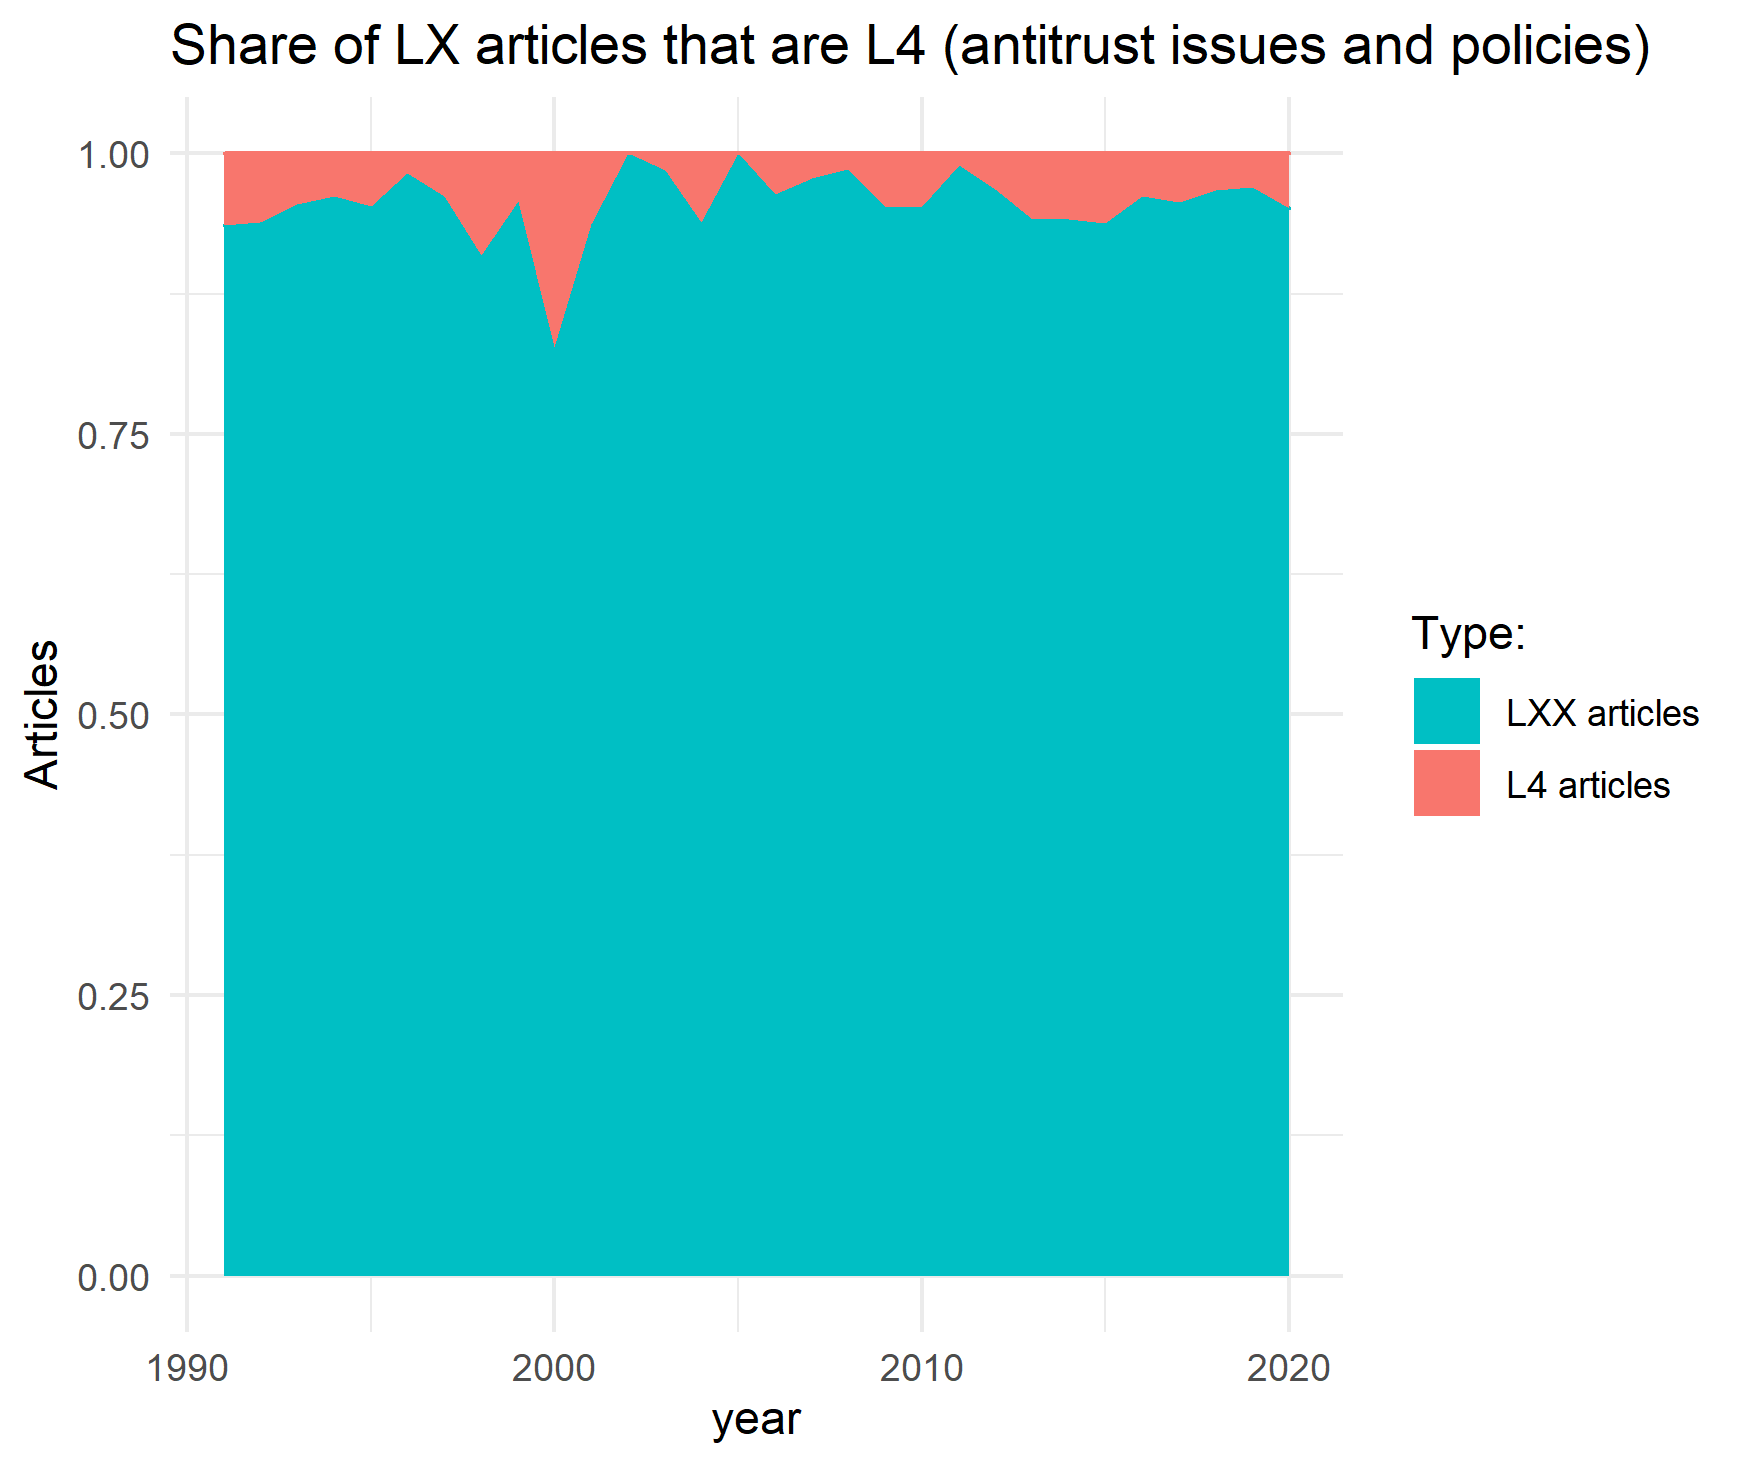
\includegraphics[width=\textwidth]{L4-vs-LXX-normalized.png}
        \caption{By share}
    \end{subfigure}
    \caption{Antitrust within Industrial Organization in the Top 5 (and RAND)}
\end{figure}

As evidenced in Figures 7(a) and 7(b), antitrust (L4) makes up a \textit{de minimis share} of even IO (LXX) papers, let alone the sample of papers published in the top journals, at large. Moreover, the number of IO publications in ECA, JPE, QJE, and RES are relatively small, and to the extent that antitrust papers do appear in the sample of journals we consider, they are highly concentrated in the \textit{RAND Journal of Economics}. Between 1991 and 2021, we identify 103 articles that are associated with antitrust (L4), just over 4\% of the IO-related (LXX) papers published in the Top 5 (and RAND) in the same period.


\begin{figure}[!ht]
    \begin{subfigure}[h]{0.49\textwidth}
        \centering
        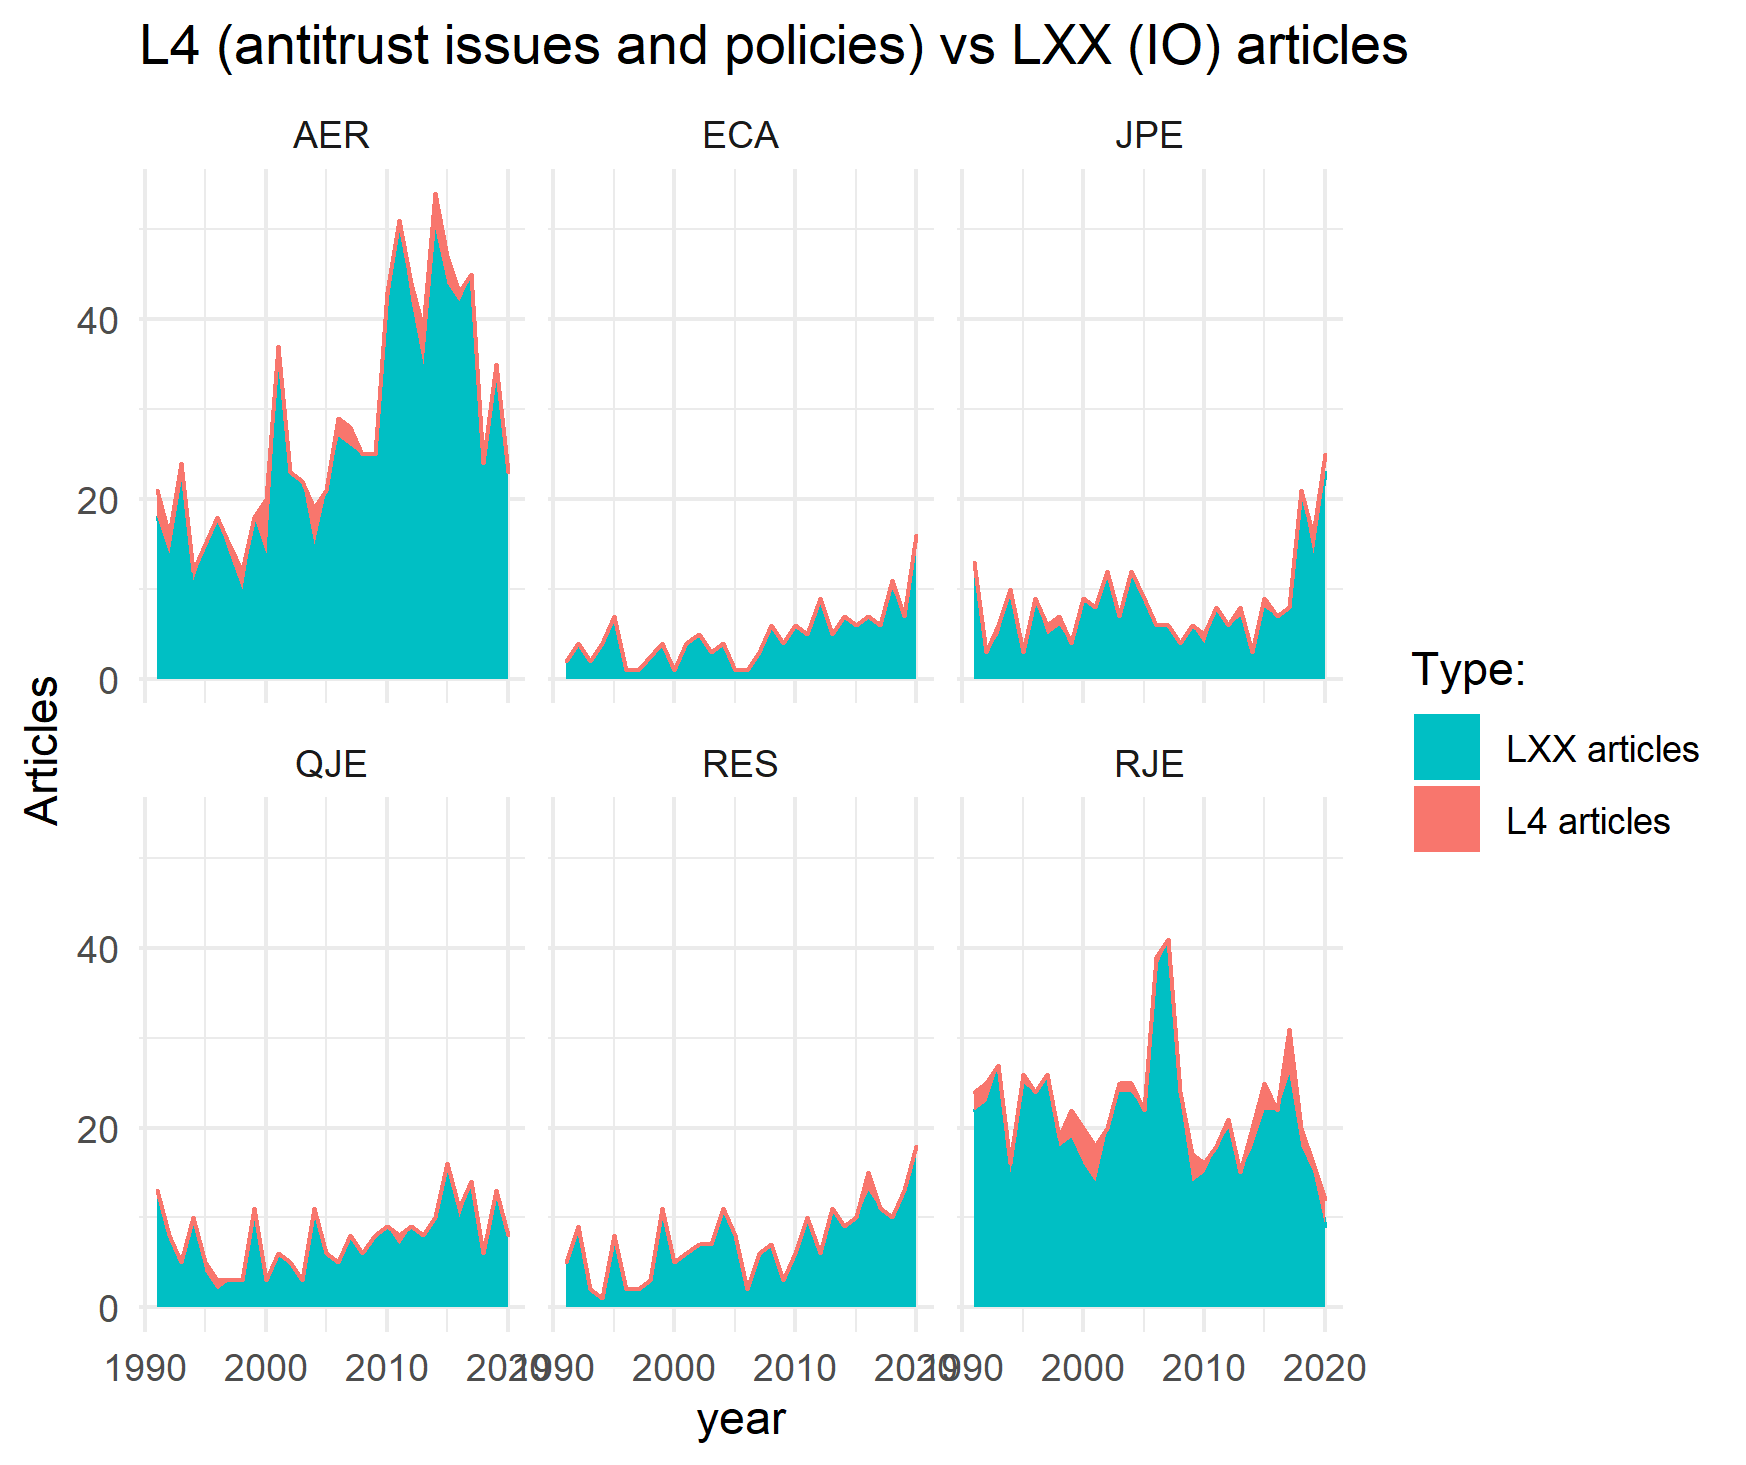
\includegraphics[width=\textwidth]{L4-vs-LXX-by-journal.png}
        \caption{By count}
    \end{subfigure}
    \hfill
    \begin{subfigure}[h]{0.49\textwidth}
        \centering
        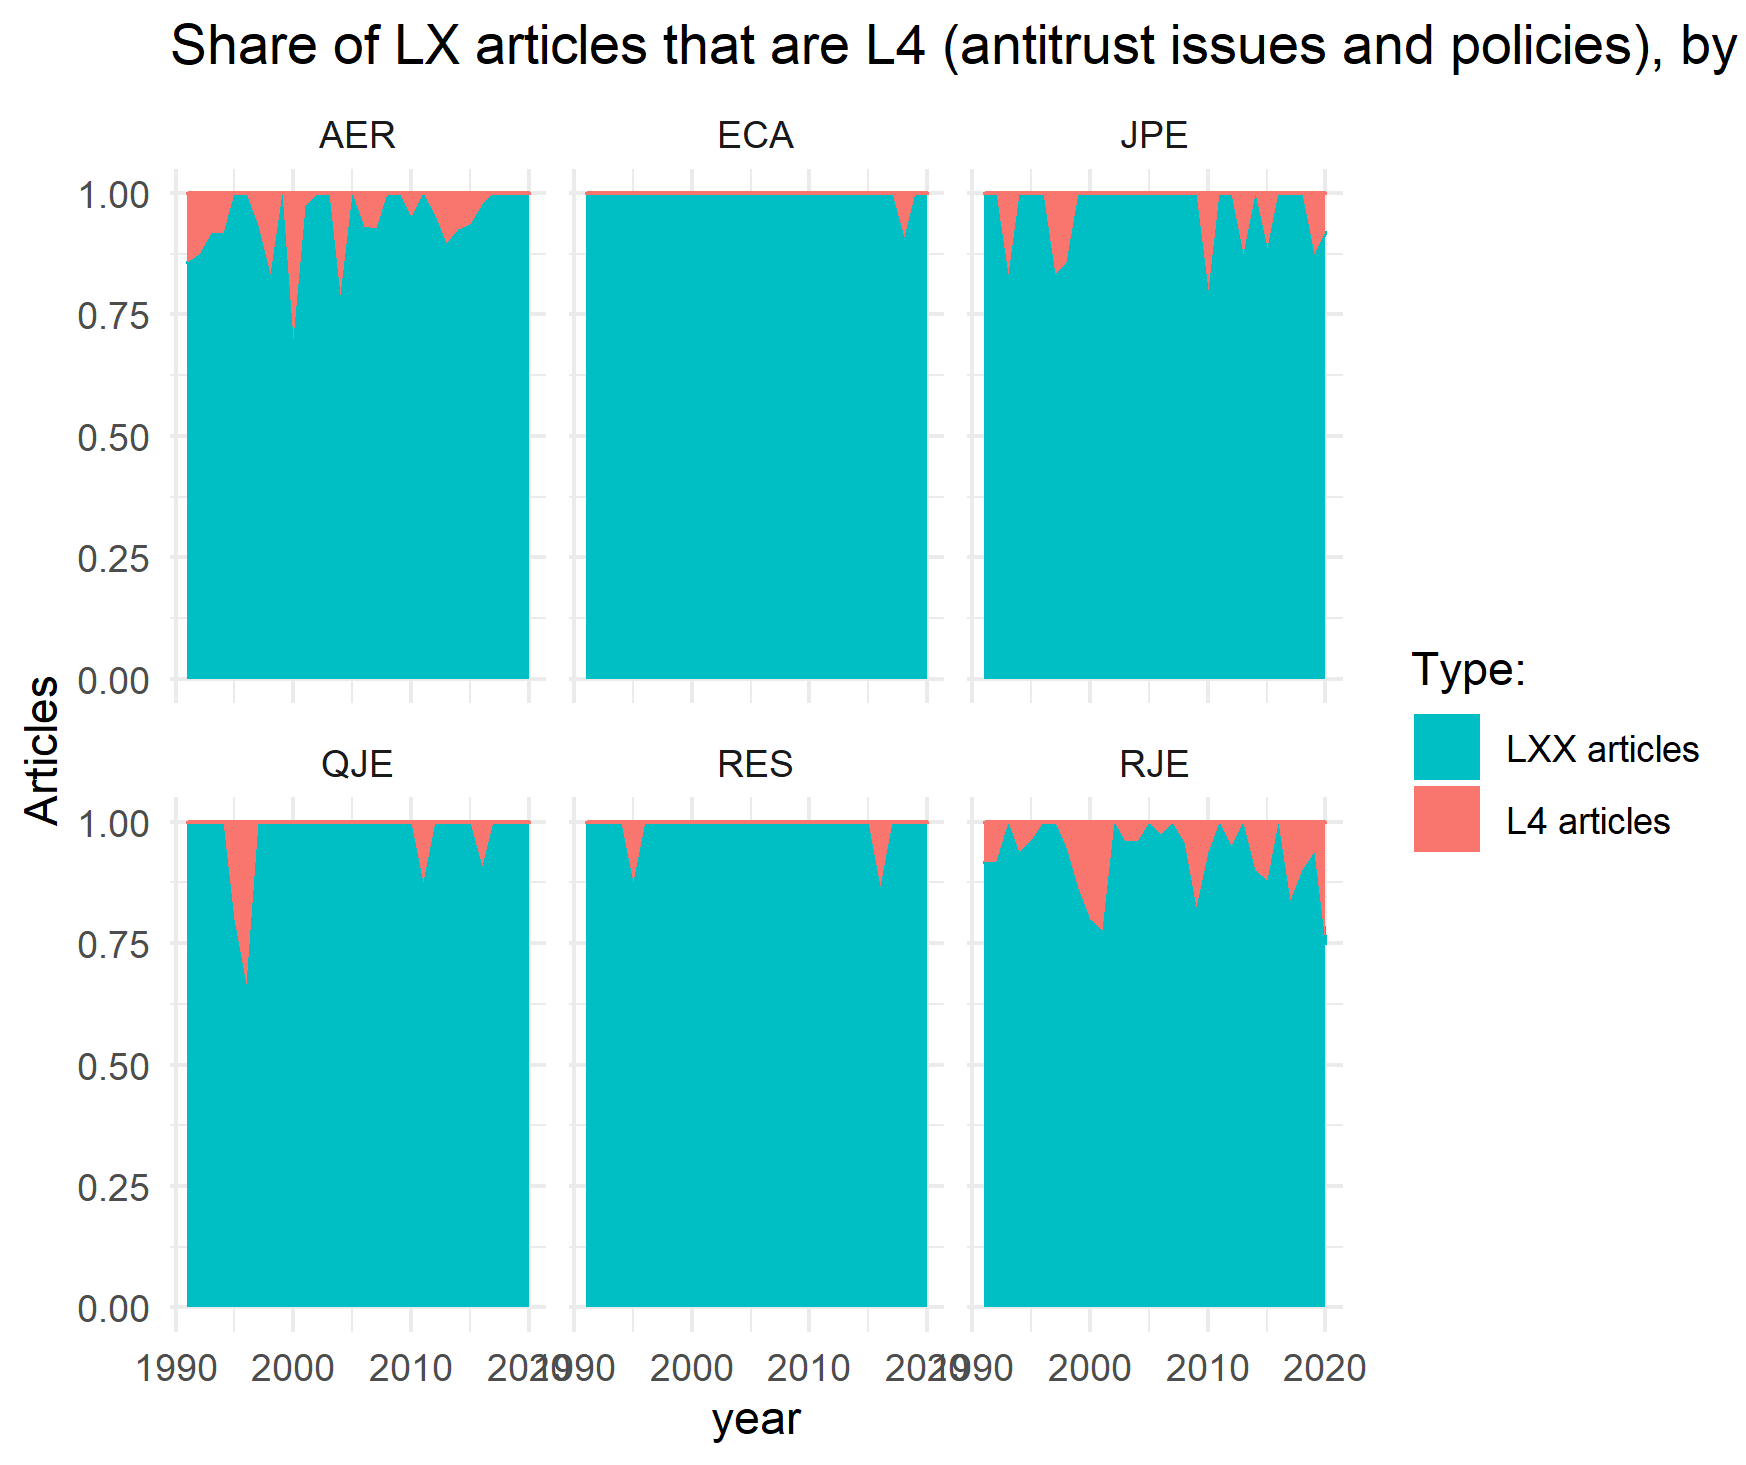
\includegraphics[width=\textwidth]{L4-vs-LXX-normalized-by_journal.png}
        \caption{By share}
    \end{subfigure}
    \caption{Antitrust within Industrial Organization in the Top 5 (and RAND), by journal}
\end{figure}

\subsection{Anti-Trust relative to Wages}
The above result -- that antitrust papers make up but a negligible share of articles published in the Top 5 (and RAND) -- we consider comparing antitrust as a topic against another area of study that has considerable policy implications: wages and compensation. We do this to see if the sub-letter level of a JEL code is too specific to identify lines of literature in the Top 5. As demonstrated in Figure 9, the considerably larger share of the Top 5 (and RAND) articles identifiable as being associated with wage studies (J3), suggests that there are strands of the literature that are identifiable with sub-letter JEL code policy areas. This again points to a dearth of antitrust papers in the most prestigious economics journals. 

\begin{figure}[!ht]
    \begin{subfigure}[h]{0.49\textwidth}
        \centering
        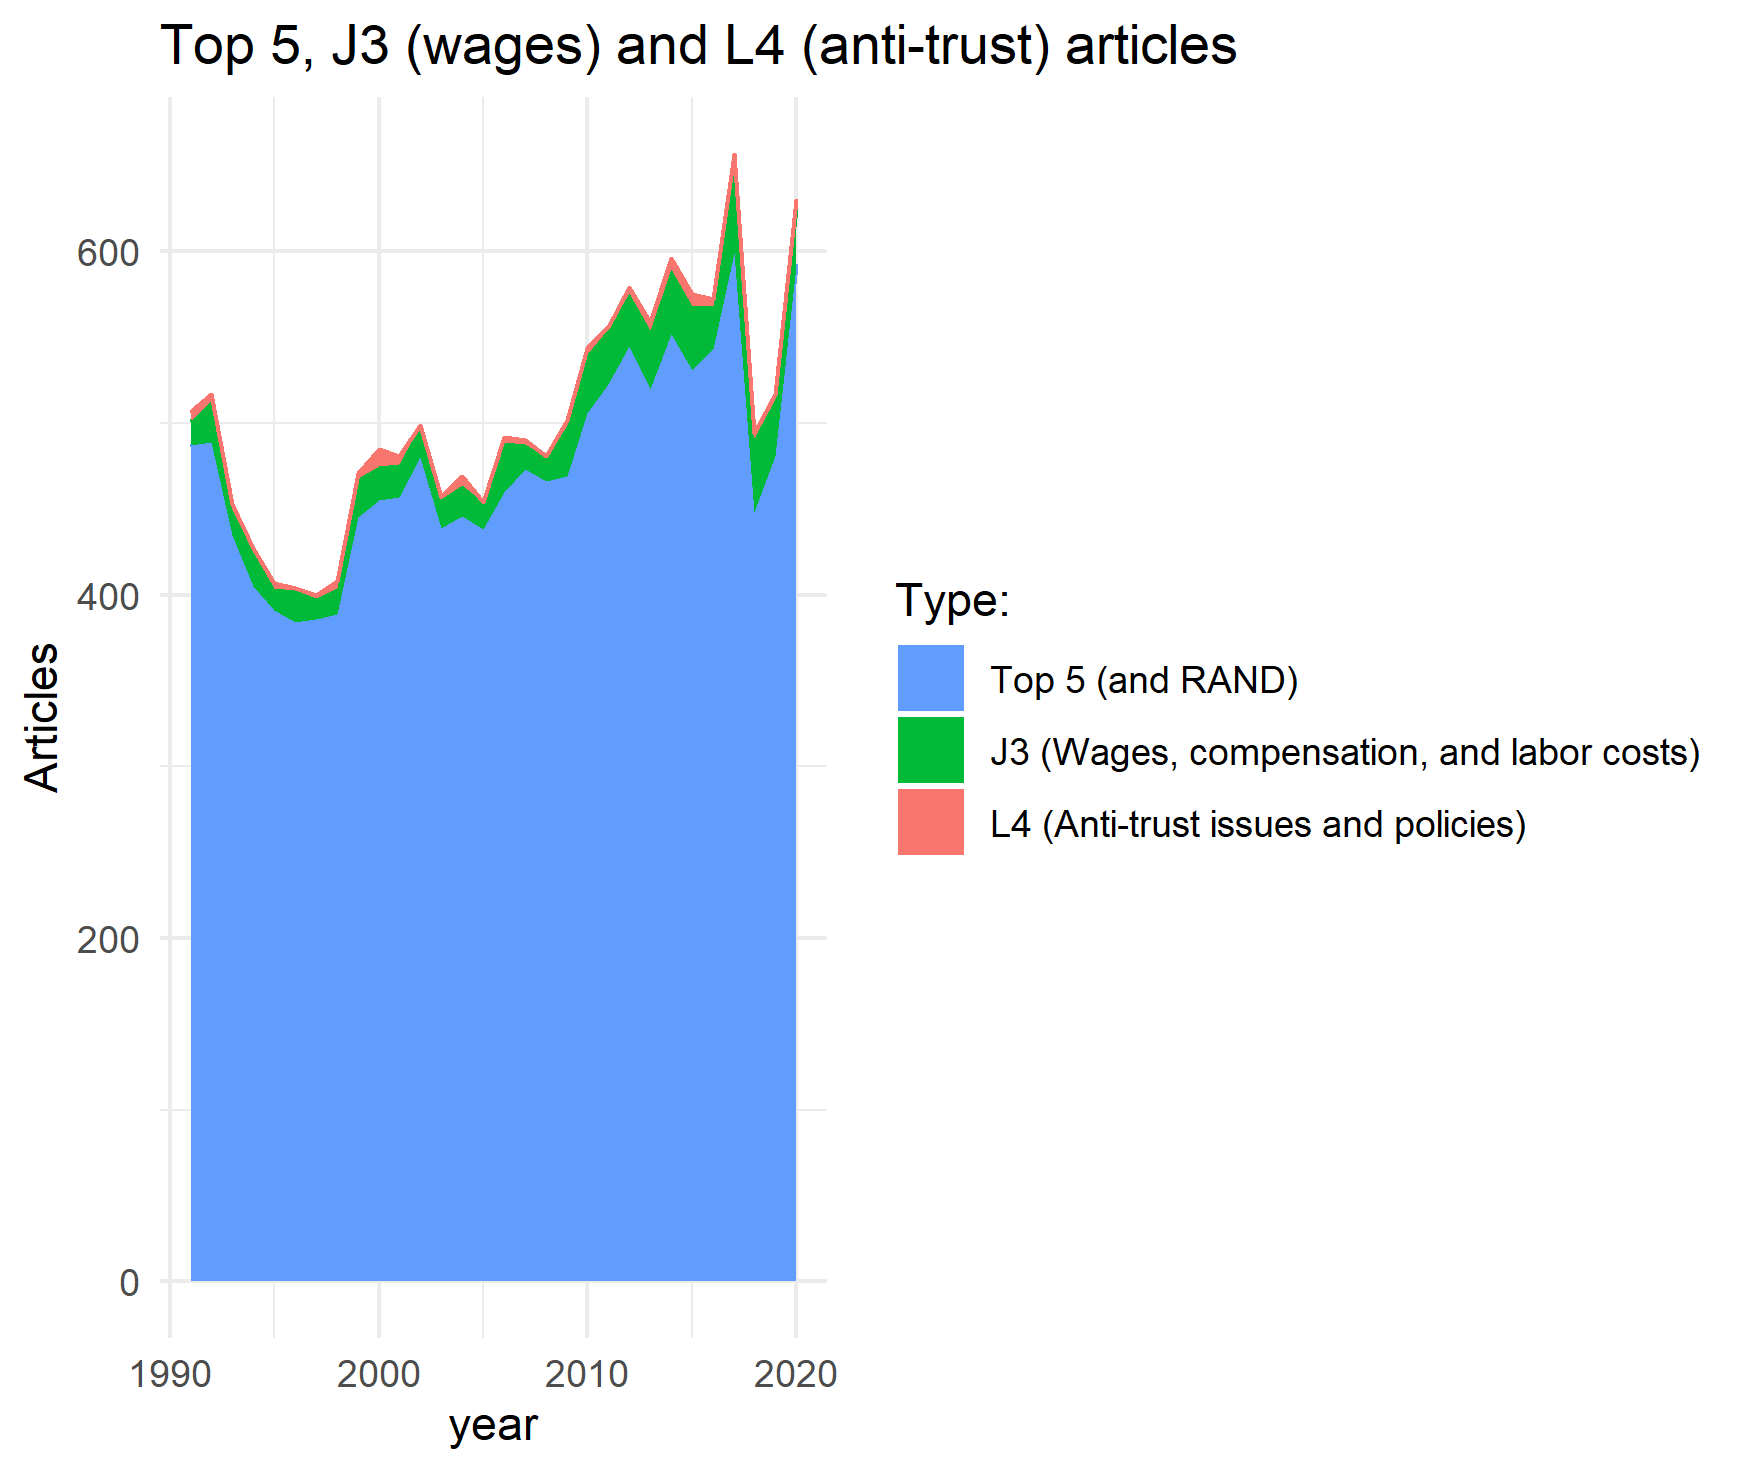
\includegraphics[width=\textwidth]{j3-l4-top5.png}
        \caption{By count}
    \end{subfigure}
    \hfill
    \begin{subfigure}[h]{0.49\textwidth}
        \centering
        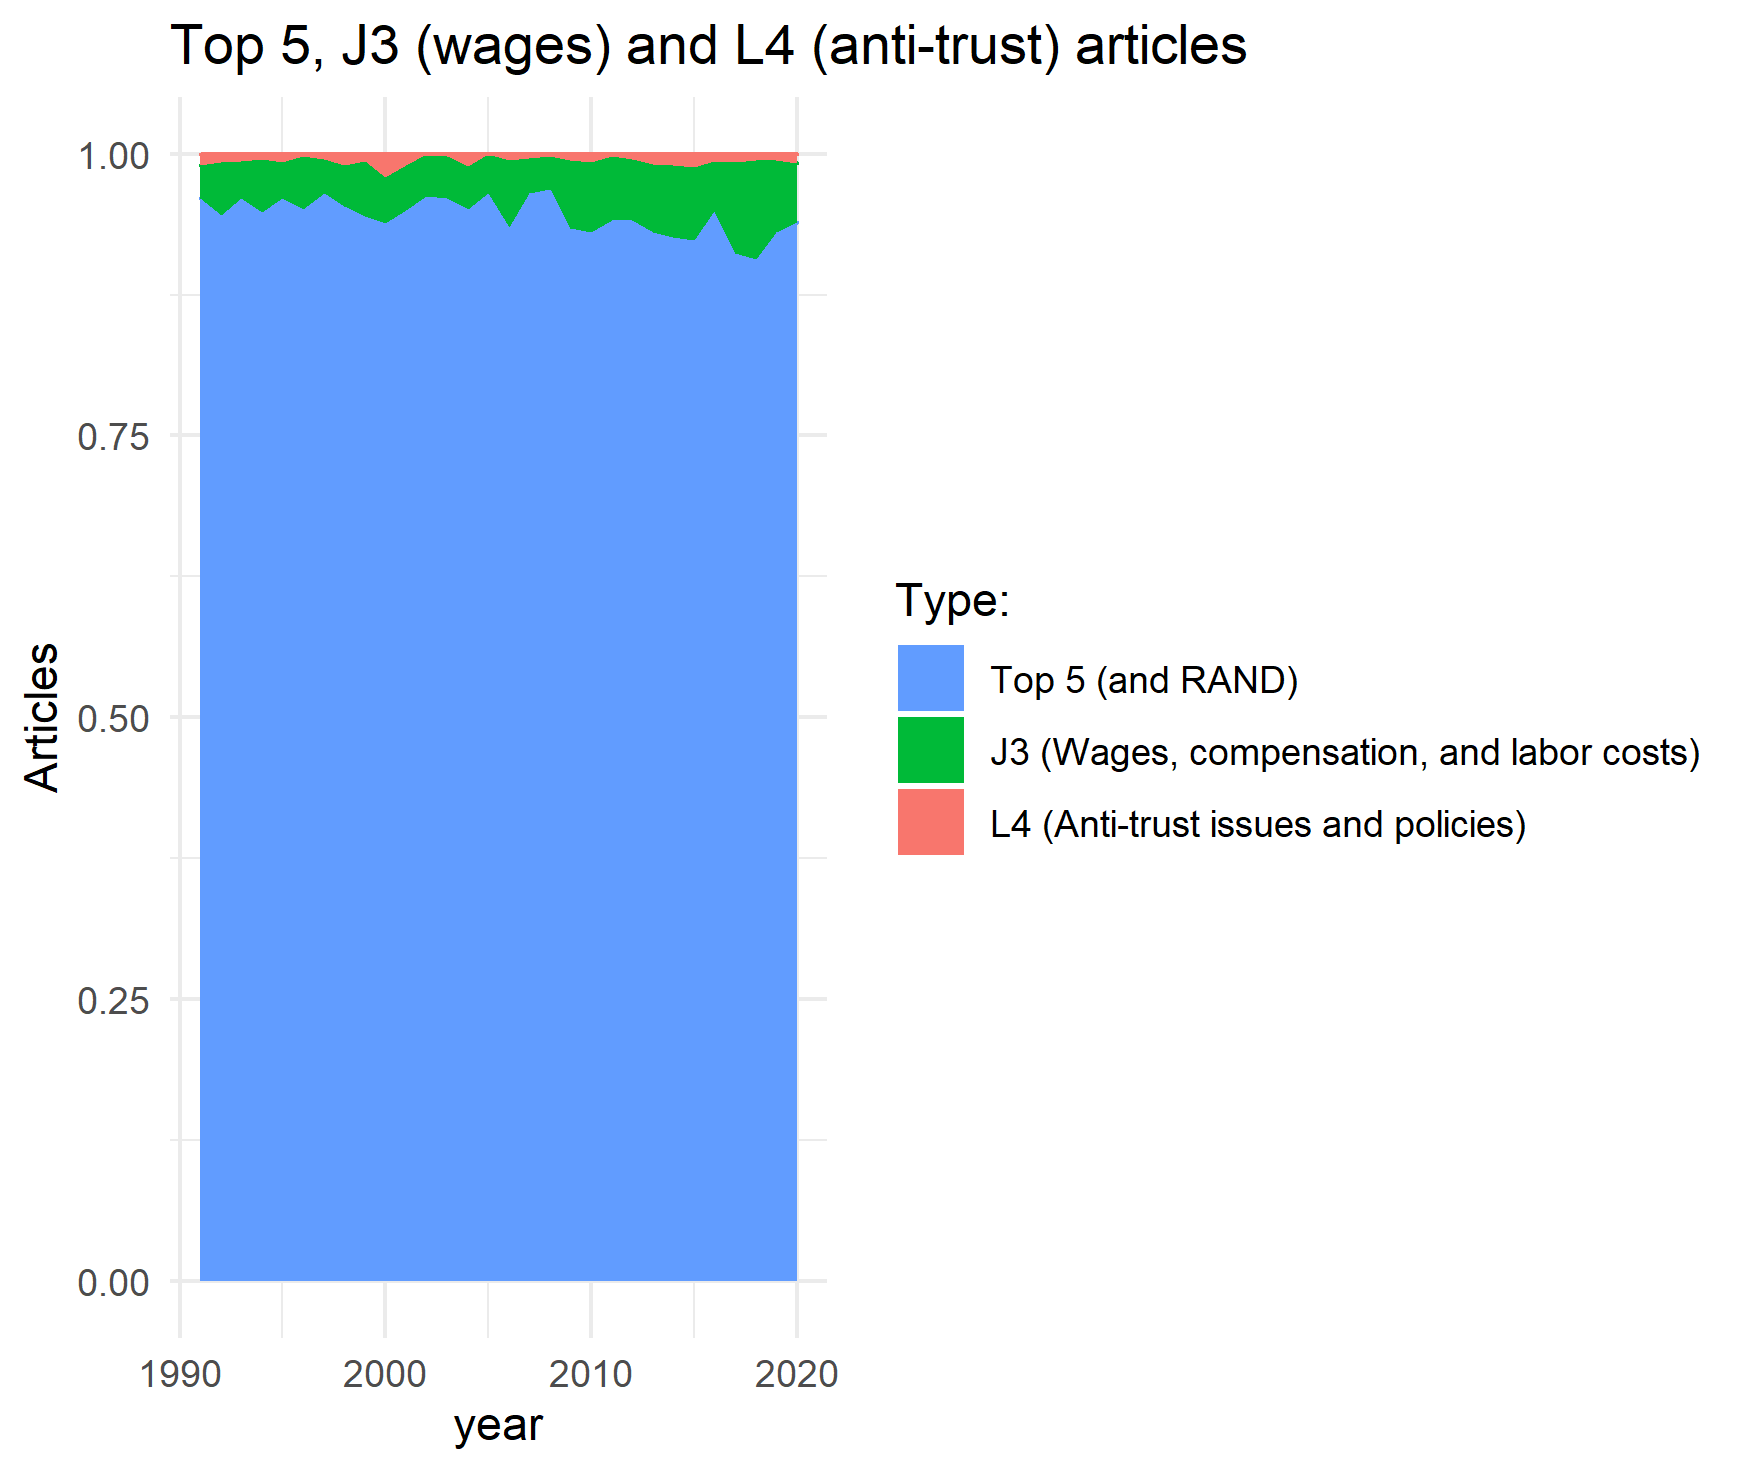
\includegraphics[width=\textwidth]{j3-l4-top5-normalized.png}
        \caption{By share}
    \end{subfigure}
    \caption{The relative frequencies of wage-studies (J3) and antitrust (L4) articles in the Top 5 (and RAND).}
\end{figure}

\newpage

\appendix
% APPENDIX A
\section{The Production of Academic Articles}
Table 1 presents the count of articles published in each of the Top 5 Journals (and RAND) during the time period of interest: 1990 to 2021. As noted above, in subsequent tables and figures, we trim the time series to cover only 1990 to 2020 so as to avoid potential complications due to incomplete indexing and/or changing JEL code formats.

% Table created by stargazer v.5.2.3 by Marek Hlavac, Social Policy Institute. E-mail: marek.hlavac at gmail.com
% Date and time: Thu, Apr 28, 2022 - 3:42:28 PM
\begin{table}[!htbp] \centering 
  \caption{Number of articles published in each of the Top 5 (and RAND), year} 
  \label{} 
\footnotesize 
\begin{tabular}{@{\extracolsep{5pt}} cccccccc} 
\\[-1.8ex]\hline 
\hline \\[-1.8ex] 
 & AER & ECA & JPE & QJE & RES & RJE & TOTAL \\ 
\hline \\[-1.8ex] 
1990 & $189$ & $66$ & $73$ & $54$ & $42$ & $40$ & $464$ \\ 
1991 & $182$ & $79$ & $67$ & $59$ & $59$ & $41$ & $487$ \\ 
1992 & $196$ & $97$ & $59$ & $56$ & $44$ & $37$ & $489$ \\ 
1993 & $190$ & $54$ & $56$ & $47$ & $48$ & $40$ & $435$ \\ 
1994 & $181$ & $53$ & $54$ & $44$ & $37$ & $36$ & $405$ \\ 
1995 & $174$ & $54$ & $50$ & $41$ & $29$ & $43$ & $391$ \\ 
1996 & $167$ & $58$ & $48$ & $41$ & $28$ & $42$ & $384$ \\ 
1997 & $162$ & $53$ & $54$ & $39$ & $30$ & $48$ & $386$ \\ 
1998 & $174$ & $46$ & $48$ & $42$ & $39$ & $40$ & $389$ \\ 
1999 & $177$ & $87$ & $63$ & $40$ & $42$ & $36$ & $445$ \\ 
2000 & $202$ & $86$ & $52$ & $43$ & $37$ & $35$ & $455$ \\ 
2001 & $201$ & $91$ & $47$ & $42$ & $38$ & $38$ & $457$ \\ 
2002 & $192$ & $116$ & $54$ & $41$ & $39$ & $38$ & $480$ \\ 
2003 & $186$ & $86$ & $47$ & $40$ & $38$ & $42$ & $439$ \\ 
2004 & $189$ & $63$ & $62$ & $41$ & $48$ & $43$ & $446$ \\ 
2005 & $202$ & $57$ & $45$ & $40$ & $46$ & $48$ & $438$ \\ 
2006 & $208$ & $70$ & $39$ & $40$ & $44$ & $59$ & $460$ \\ 
2007 & $214$ & $70$ & $34$ & $44$ & $48$ & $63$ & $473$ \\ 
2008 & $215$ & $70$ & $37$ & $41$ & $51$ & $52$ & $466$ \\ 
2009 & $232$ & $76$ & $32$ & $44$ & $50$ & $35$ & $469$ \\ 
2010 & $257$ & $86$ & $32$ & $44$ & $53$ & $34$ & $506$ \\ 
2011 & $291$ & $70$ & $33$ & $47$ & $50$ & $32$ & $523$ \\ 
2012 & $281$ & $109$ & $30$ & $41$ & $52$ & $32$ & $545$ \\ 
2013 & $260$ & $84$ & $35$ & $56$ & $53$ & $32$ & $520$ \\ 
2014 & $286$ & $89$ & $34$ & $56$ & $52$ & $35$ & $552$ \\ 
2015 & $272$ & $93$ & $37$ & $45$ & $48$ & $36$ & $531$ \\ 
2016 & $286$ & $80$ & $41$ & $40$ & $53$ & $43$ & $543$ \\ 
2017 & $287$ & $89$ & $76$ & $43$ & $57$ & $47$ & $599$ \\ 
2018 & $125$ & $90$ & $85$ & $40$ & $68$ & $40$ & $448$ \\ 
2019 & $139$ & $86$ & $97$ & $41$ & $78$ & $40$ & $481$ \\ 
2020 & $129$ & $116$ & $176$ & $41$ & $81$ & $49$ & $592$ \\ 
2021 & $127$ & $109$ & $101$ & $24$ & $28$ & $11$ & $400$ \\ 
\hline \\[-1.8ex] 
\end{tabular} 
\end{table} 



Table 2 presents the ordinal ranking of the top five JEL categories in each journal for selected years. In the case that Industrial Organization (L) is \textit{not} one of the top 5 categories, it and its ordinal ranking in that journal-year are given as a sixth entry. Note that when creating this ordinal ranking the \textit{weighted} frequencies of JEL codes are used.  
\newpage
\begin{landscape}
    \thispagestyle{empty}
    
% Table created by stargazer v.5.2.3 by Marek Hlavac, Social Policy Institute. E-mail: marek.hlavac at gmail.com
% Date and time: Fri, May 06, 2022 - 3:01:46 PM
\begin{table}[h] \centering 
  \caption{Ordinal ranking of most frequently (weighted) appearing JEL codes in the Top 5 for selected years} 
  \label{} 
\begin{adjustbox}{max width = \textwidth}
\scriptsize 
\begin{tabular}{@{\extracolsep{5pt}} lllllll} 
\\[-1.8ex]\hline 
\hline \\[-1.8ex] \multicolumn{7}{c}{Publication : \textit{American Economic Review}} \\
 \cline{1-7} \\
1991 & 1995 & 2000 & 2005 & 2010 & 2015 & 2020 \\ 
\hline \\[-1.8ex] 
1. D: Micro & 1. J: Labor Economics & 1. J: Labor Economics & 1. D: Micro & 1. D: Micro & 1. D: Micro & 1. D: Micro \\ 
2. E: Macro and Monetary & 2. D: Micro & 2. E: Macro and Monetary & 2. J: Labor Economics & 2. Y: Misc. & 2. J: Labor Economics & 2. E: Macro and Monetary \\ 
3. J: Labor Economics & 3. I: Health, Education, and Welfare & 3. D: Micro & 3. I: Health, Education, and Welfare & 3. E: Macro and Monetary & 3. Y: Misc. & 3. C: Methods \\ 
4. H: Public & 4. E: Macro and Monetary & 4. O: Development and Technology & 4. E: Macro and Monetary & 4. J: Labor Economics & 4. E: Macro and Monetary & 4. I: Health, Education, and Welfare \\ 
5. L: Industrial Organization & 5. F: International & 5. F: International & 5. F: International & 5. F: International & 5. I: Health, Education, and Welfare & 5. J: Labor Economics \\ 
 & 7. L: Industrial Organization & 6. L: Industrial Organization & 7. L: Industrial Organization & 7. L: Industrial Organization & 7. L: Industrial Organization & 11. L: Industrial Organization \\ 
 \multicolumn{7}{c}{Publication : \textit{Econometrica}} \\
 \cline{1-7} \\
1991 & 1995 & 2000 & 2005 & 2010 & 2015 & 2020 \\ 
\hline \\[-1.8ex] 
1. C: Methods & 1. C: Methods & 1. C: Methods & 1. C: Methods & 1. D: Micro & 1. D: Micro & 1. D: Micro \\ 
2. D: Micro & 2. D: Micro & 2. D: Micro & 2. D: Micro & 2. C: Methods & 2. C: Methods & 2. C: Methods \\ 
3. E: Macro and Monetary & 3. L: Industrial Organization & 3. E: Macro and Monetary & 3. E: Macro and Monetary & 3. J: Labor Economics & 3. Y: Misc. & 3. J: Labor Economics \\ 
4. F: International & 4. I: Health, Education, and Welfare & 4. G: Finance & 4. J: Labor Economics & 4. L: Industrial Organization & 4. J: Labor Economics & 4. E: Macro and Monetary \\ 
5. J: Labor Economics & 5. H: Public & 5. O: Development and Technology & 5. I: Health, Education, and Welfare & 5. G: Finance & 5. G: Finance & 5. O: Development and Technology \\ 
7. L: Industrial Organization &  & 7. L: Industrial Organization & 10. L: Industrial Organization &  & 9. L: Industrial Organization & 6. L: Industrial Organization \\ 

 \multicolumn{7}{c}{Publication : \textit{Journal of Political Economy}} \\
 \cline{1-7} \\
1991 & 1995 & 2000 & 2005 & 2010 & 2015 & 2020 \\ 
\hline \\[-1.8ex] 
1. D: Micro & 1. D: Micro & 1. D: Micro & 1. D: Micro & 1. D: Micro & 1. D: Micro & 1. D: Micro \\ 
2. L: Industrial Organization & 2. O: Development and Technology & 2. J: Labor Economics & 2. J: Labor Economics & 2. J: Labor Economics & 2. I: Health, Education, and Welfare & 2. J: Labor Economics \\ 
3. E: Macro and Monetary & 3. I: Health, Education, and Welfare & 3. L: Industrial Organization & 3. L: Industrial Organization & 3. I: Health, Education, and Welfare & 3. J: Labor Economics & 3. G: Finance \\ 
4. J: Labor Economics & 4. J: Labor Economics & 4. G: Finance & 4. E: Macro and Monetary & 4. O: Development and Technology & 4. L: Industrial Organization & 4. I: Health, Education, and Welfare \\ 
5. O: Development and Technology & 5. H: Public & 5. O: Development and Technology & 5. F: International & 5. L: Industrial Organization & 5. E: Macro and Monetary & 5. L: Industrial Organization \\ 
 & 11. L: Industrial Organization &  &  &  &  &  \\ 

 \multicolumn{7}{c}{Publication : \textit{Quarterly Journal of Economics}} \\
 \cline{1-7} \\
1991 & 1995 & 2000 & 2005 & 2010 & 2015 & 2020 \\ 
\hline \\[-1.8ex] 
1. J: Labor Economics & 1. D: Micro & 1. D: Micro & 1. D: Micro & 1. D: Micro & 1. D: Micro & 1. D: Micro \\ 
2. O: Development and Technology & 2. E: Macro and Monetary & 2. I: Health, Education, and Welfare & 2. J: Labor Economics & 2. J: Labor Economics & 2. J: Labor Economics & 2. E: Macro and Monetary \\ 
3. D: Micro & 3. J: Labor Economics & 3. J: Labor Economics & 3. O: Development and Technology & 3. I: Health, Education, and Welfare & 3. L: Industrial Organization & 3. J: Labor Economics \\ 
4. L: Industrial Organization & 4. O: Development and Technology & 4. E: Macro and Monetary & 4. G: Finance & 4. F: International & 4. I: Health, Education, and Welfare & 4. I: Health, Education, and Welfare \\ 
5. F: International & 5. L: Industrial Organization & 5. Z: Special Topics & 5. L: Industrial Organization & 5. G: Finance & 5. O: Development and Technology & 5. O: Development and Technology \\ 
 &  & 9. L: Industrial Organization &  & 7. L: Industrial Organization &  & 8. L: Industrial Organization \\ 

 \multicolumn{7}{c}{Publication : \textit{Review of Economic Studies}} \\
 \cline{1-7} \\
1991 & 1995 & 2000 & 2005 & 2010 & 2015 & 2020 \\ 
\hline \\[-1.8ex] 
1. D: Micro & 1. D: Micro & 1. D: Micro & 1. D: Micro & 1. D: Micro & 1. D: Micro & 1. D: Micro \\ 
2. C: Methods & 2. L: Industrial Organization & 2. C: Methods & 2. C: Methods & 2. C: Methods & 2. J: Labor Economics & 2. G: Finance \\ 
3. F: International & 3. J: Labor Economics & 3. J: Labor Economics & 3. E: Macro and Monetary & 3. J: Labor Economics & 3. F: International & 3. J: Labor Economics \\ 
4. J: Labor Economics & 4. G: Finance & 4. L: Industrial Organization & 4. L: Industrial Organization & 4. H: Public & 4. C: Methods & 4. E: Macro and Monetary \\ 
5. E: Macro and Monetary & 5. C: Methods & 5. H: Public & 5. G: Finance & 5. E: Macro and Monetary & 5. G: Finance & 5. I: Health, Education, and Welfare \\ 
8. L: Industrial Organization &  &  &  & 7. L: Industrial Organization & 7. L: Industrial Organization & 7. L: Industrial Organization \\ 
\hline 
\end{tabular} 
\end{adjustbox} 
\end{table} 

\end{landscape}

\section{The Role of Industrial Organization}
Tables 3 and 4 present the count and share of Industrial Organization articles in the Top 5 (and RAND), by year. Whereas Table 3 presents the IO count and share aggregated over all of the journals, by year, Table 4 presents the count of all articles published and the share of those that are IO-related, for each journal, by year. Note that for both Tables 3 and 4, the IO Share figures are calculated using the \textit{absolute} frequencies \textsc{not} the weighted frequencies.

% Table created by stargazer v.5.2.3 by Marek Hlavac, Social Policy Institute. E-mail: marek.hlavac at gmail.com
% Date and time: Fri, Apr 29, 2022 - 1:00:37 PM
\begin{table}[!htbp] \centering 
  \caption{The count and share of Industrial Organization articles in the Top 5 (and RAND), by year} 
  \label{} 
\footnotesize 
\begin{tabular}{@{\extracolsep{5pt}} cccc} 
\\[-1.8ex]\hline 
\hline \\[-1.8ex] 
 & IO (LXX) & Top 5 (and RAND) & IO Share \\ 
\hline \\[-1.8ex] 
1991 & $78$ & $487$ & 16.0\% \\ 
1992 & $65$ & $489$ & 13.3\% \\ 
1993 & $66$ & $435$ & 15.2\% \\ 
1994 & $53$ & $405$ & 13.1\% \\ 
1995 & $64$ & $391$ & 16.4\% \\ 
1996 & $57$ & $384$ & 14.8\% \\ 
1997 & $53$ & $386$ & 13.7\% \\ 
1998 & $44$ & $389$ & 11.3\% \\ 
1999 & $70$ & $445$ & 15.7\% \\ 
2000 & $58$ & $455$ & 12.7\% \\ 
2001 & $79$ & $457$ & 17.3\% \\ 
2002 & $72$ & $480$ & 15.0\% \\ 
2003 & $67$ & $439$ & 15.3\% \\ 
2004 & $82$ & $446$ & 18.4\% \\ 
2005 & $67$ & $438$ & 15.3\% \\ 
2006 & $82$ & $460$ & 17.8\% \\ 
2007 & $92$ & $473$ & 19.5\% \\ 
2008 & $72$ & $466$ & 15.5\% \\ 
2009 & $63$ & $469$ & 13.4\% \\ 
2010 & $85$ & $506$ & 16.8\% \\ 
2011 & $100$ & $523$ & 19.1\% \\ 
2012 & $95$ & $545$ & 17.4\% \\ 
2013 & $86$ & $520$ & 16.5\% \\ 
2014 & $103$ & $552$ & 18.7\% \\ 
2015 & $113$ & $531$ & 21.3\% \\ 
2016 & $105$ & $543$ & 19.3\% \\ 
2017 & $115$ & $599$ & 19.2\% \\ 
2018 & $92$ & $448$ & 20.5\% \\ 
2019 & $100$ & $481$ & 20.8\% \\ 
2020 & $102$ & $592$ & 17.2\% \\ 
\hline \\[-1.8ex] 
\end{tabular} 
\end{table} 



% Table created by stargazer v.5.2.3 by Marek Hlavac, Social Policy Institute. E-mail: marek.hlavac at gmail.com
% Date and time: Fri, Apr 29, 2022 - 1:37:53 PM
\begin{table}[!htbp] \centering 
  \caption{Share of publications that are IO-related, by year} 
  \label{} 
\begin{adjustbox}{max width = \textwidth}
\footnotesize 
\begin{tabular}{@{\extracolsep{2pt}} ccccccccccccc} 
\\[-1.8ex]\hline 
\hline \\[-1.8ex] & \multicolumn{2}{c}{\textit{AER}}& \multicolumn{2}{c}{\textit{ECA}}& \multicolumn{2}{c}{\textit{JPE}}& \multicolumn{2}{c}{\textit{QJE}}& \multicolumn{2}{c}{\textit{RES}}& \multicolumn{2}{c}{\textit{RJE}}\\ 
\cline{2-3}\cline{4-5}\cline{6-7}\cline{8-9}\cline{10-11}\cline{12-13}\\ 
 & Count & IO Share & Count & IO Share & Count & IO Share & Count & IO Share & Count & IO Share & Count & IO Share \\ 
\hline \\[-1.8ex] 
1991 & $182$ & 11.54\% & $79$ & 2.53\% & $67$ & 19.40\% & $59$ & 22.03\% & $59$ & 8.47\% & $41$ & 58.54\% \\ 
1992 & $196$ & 8.16\% & $97$ & 4.12\% & $59$ & 5.08\% & $56$ & 14.29\% & $44$ & 20.45\% & $37$ & 67.57\% \\ 
1993 & $190$ & 12.63\% & $54$ & 3.70\% & $56$ & 10.71\% & $47$ & 10.64\% & $48$ & 4.17\% & $40$ & 67.50\% \\ 
1994 & $181$ & 6.63\% & $53$ & 7.55\% & $54$ & 18.52\% & $44$ & 22.73\% & $37$ & 2.70\% & $36$ & 44.44\% \\ 
1995 & $174$ & 8.62\% & $54$ & 12.96\% & $50$ & 6.00\% & $41$ & 12.20\% & $29$ & 27.59\% & $43$ & 60.47\% \\ 
1996 & $167$ & 10.78\% & $58$ & 1.72\% & $48$ & 18.75\% & $41$ & 7.32\% & $28$ & 7.14\% & $42$ & 57.14\% \\ 
1997 & $162$ & 9.26\% & $53$ & 1.89\% & $54$ & 11.11\% & $39$ & 7.69\% & $30$ & 6.67\% & $48$ & 54.17\% \\ 
1998 & $174$ & 6.90\% & $46$ & 0.00\% & $48$ & 14.58\% & $42$ & 7.14\% & $39$ & 7.69\% & $40$ & 47.50\% \\ 
1999 & $177$ & 10.17\% & $87$ & 4.60\% & $63$ & 6.35\% & $40$ & 27.50\% & $42$ & 26.19\% & $36$ & 61.11\% \\ 
2000 & $202$ & 9.90\% & $86$ & 1.16\% & $52$ & 17.31\% & $43$ & 6.98\% & $37$ & 13.51\% & $35$ & 57.14\% \\ 
2001 & $201$ & 18.41\% & $91$ & 4.40\% & $47$ & 17.02\% & $42$ & 14.29\% & $38$ & 15.79\% & $38$ & 47.37\% \\ 
2002 & $192$ & 11.98\% & $116$ & 4.31\% & $54$ & 22.22\% & $41$ & 12.20\% & $39$ & 17.95\% & $38$ & 52.63\% \\ 
2003 & $186$ & 11.83\% & $86$ & 3.49\% & $47$ & 14.89\% & $40$ & 7.50\% & $38$ & 18.42\% & $42$ & 59.52\% \\ 
2004 & $189$ & 10.05\% & $63$ & 6.35\% & $62$ & 19.35\% & $41$ & 26.83\% & $48$ & 22.92\% & $43$ & 58.14\% \\ 
2005 & $202$ & 10.40\% & $57$ & 1.75\% & $45$ & 20.00\% & $40$ & 15.00\% & $46$ & 17.39\% & $48$ & 45.83\% \\ 
2006 & $208$ & 13.94\% & $70$ & 1.43\% & $39$ & 15.38\% & $40$ & 12.50\% & $44$ & 4.55\% & $59$ & 66.10\% \\ 
2007 & $214$ & 13.08\% & $70$ & 4.29\% & $34$ & 17.65\% & $44$ & 18.18\% & $48$ & 12.50\% & $63$ & 65.08\% \\ 
2008 & $215$ & 11.63\% & $70$ & 8.57\% & $37$ & 10.81\% & $41$ & 14.63\% & $51$ & 13.73\% & $52$ & 46.15\% \\ 
2009 & $232$ & 10.78\% & $76$ & 5.26\% & $32$ & 18.75\% & $44$ & 18.18\% & $50$ & 6.00\% & $35$ & 48.57\% \\ 
2010 & $257$ & 16.73\% & $86$ & 6.98\% & $32$ & 15.62\% & $44$ & 20.45\% & $53$ & 11.32\% & $34$ & 47.06\% \\ 
2011 & $291$ & 17.53\% & $70$ & 7.14\% & $33$ & 24.24\% & $47$ & 17.02\% & $50$ & 20.00\% & $32$ & 56.25\% \\ 
2012 & $281$ & 15.66\% & $109$ & 8.26\% & $30$ & 20.00\% & $41$ & 21.95\% & $52$ & 11.54\% & $32$ & 65.62\% \\ 
2013 & $260$ & 15.00\% & $84$ & 5.95\% & $35$ & 22.86\% & $56$ & 14.29\% & $53$ & 20.75\% & $32$ & 46.88\% \\ 
2014 & $286$ & 18.88\% & $89$ & 7.87\% & $34$ & 8.82\% & $56$ & 17.86\% & $52$ & 17.31\% & $35$ & 57.14\% \\ 
2015 & $272$ & 17.28\% & $93$ & 6.45\% & $37$ & 24.32\% & $45$ & 35.56\% & $48$ & 20.83\% & $36$ & 69.44\% \\ 
2016 & $286$ & 15.03\% & $80$ & 8.75\% & $41$ & 17.07\% & $40$ & 27.50\% & $53$ & 28.30\% & $43$ & 51.16\% \\ 
2017 & $287$ & 15.68\% & $89$ & 6.74\% & $76$ & 10.53\% & $43$ & 32.56\% & $57$ & 19.30\% & $47$ & 65.96\% \\ 
2018 & $125$ & 19.20\% & $90$ & 12.22\% & $85$ & 24.71\% & $40$ & 15.00\% & $68$ & 14.71\% & $40$ & 50.00\% \\ 
2019 & $139$ & 25.18\% & $86$ & 8.14\% & $97$ & 16.49\% & $41$ & 31.71\% & $78$ & 16.67\% & $40$ & 40.00\% \\ 
2020 & $129$ & 17.83\% & $116$ & 13.79\% & $176$ & 14.20\% & $41$ & 19.51\% & $81$ & 22.22\% & $49$ & 24.49\% \\ 
\hline \\[-1.8ex] 
\end{tabular} 
\end{adjustbox} 
\end{table} 


\newpage
\section{Miscellaneous}
We additionally try to investigate the frequency of antitrust or related IO topics in the Top 5 (and RAND) by naively examining the abstracts of those papers. A paper is counted if a pattern of interest is matched in the abstract. We use open-ended patterns wherever possible to maximize the chances of identify a match. For example, we construct the monopoly pattern as ``monopol'' so that a regex match would be identified not only for ``monopoly'' but also for ``monopolization.'' The results of this effort are presented in Table 5.


\begin{table}[h] \centering 
    \caption{Appearance of miscellaneous terms in article abstracts, by journal} 
    \label{} 
    \begin{adjustbox}{max width=\textwidth}
        \begin{tabular}{@{\extracolsep{5pt}} ccccccccccc} 
            \\[-1.8ex]\hline 
            \hline \\[-1.8ex]
            & \multicolumn{6}{c}{\textit{Abstract contains:}} & \multicolumn{4}{c}{\textit{JEL Code}} \\ 
          \cline{2-7} \cline{8-11} \\
            Publication & Anti Trust & Market Power & Anti Competitive & Monopoly & Merger & Cartel & L & K & L4 & K21 \\ 
            \hline \\[-1.8ex] 
            AER & 11 & 25 & 6 & 52 & 30 & 15 & 869 & 216 & 43 & 24 \\ 
            ECA & 1 & 8 & 1 & 22 & 4 & 3 & 154 & 20 & 1 & 7 \\ 
            JPE & 5 & 16 & 1 & 27 & 7 & 5 & 279 & 78 & 12 & 7 \\ 
            QJE & 1 & 12 & 1 & 25 & 8 & 0 & 239 & 60 & 4 & 0 \\ 
            RES & 2 & 9 & 1 & 52 & 5 & 2 & 228 & 39 & 3 & 1 \\ 
            RJE & 21 & 37 & 13 & 113 & 48 & 16 & 679 & 87 & 43 & 15 \\ 
            TOTAL & 41 & 107 & 23 & 291 & 102 & 41 & 2448 & 500 & 106 & 54 \\ 
            \hline \\[-1.8ex] 
        \end{tabular}    
    \end{adjustbox}
\end{table} 



\end{document}